\section{Individual sources of Jet Energy Correction uncertainties}
\label{sec:JECs}

\begin{figure}[!hbtp]
%\begin{center}
\hspace*{-5mm}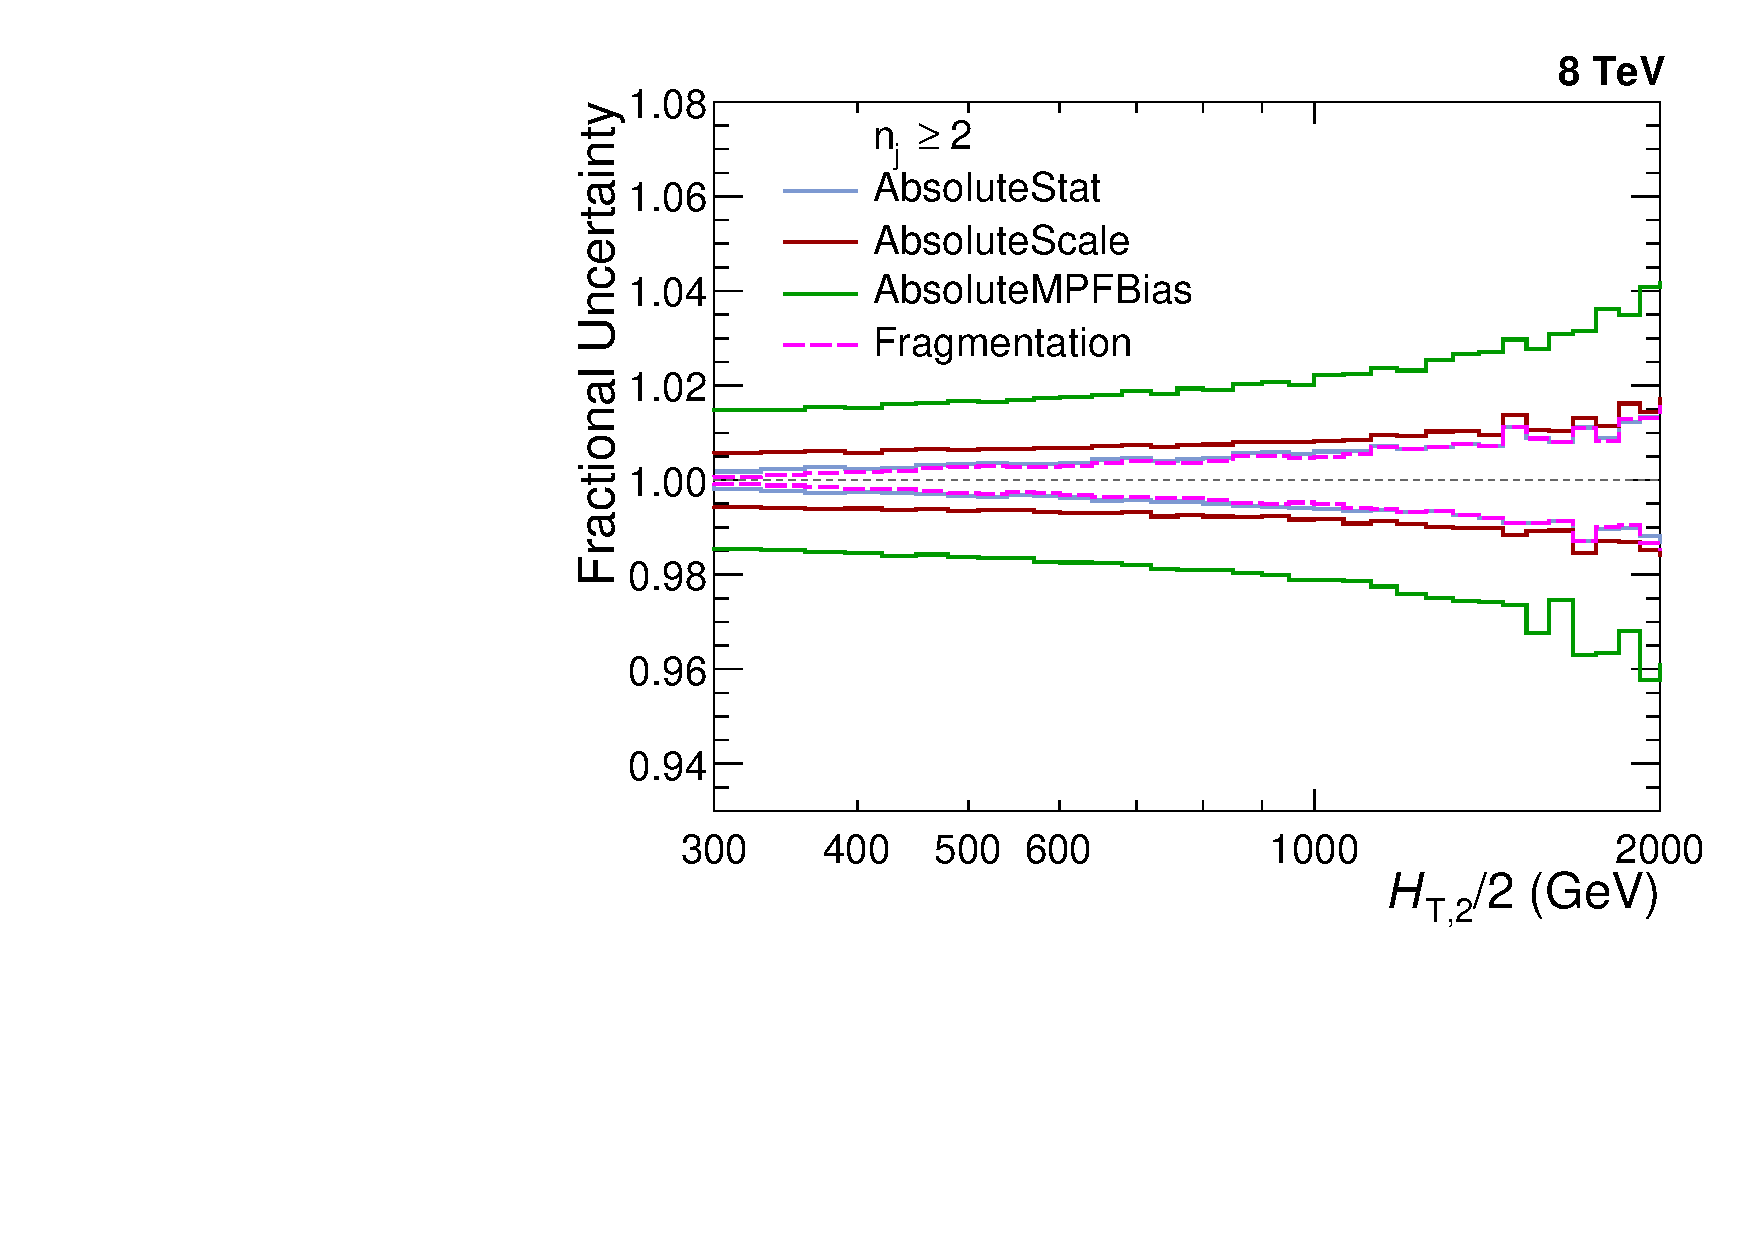
\includegraphics[width=0.51\textwidth]{/home/anter/Desktop/Thesis/Plots_HT_2_150/Single/MC_Macro_Plot_All_2_HT_2_Unc_Abs_1.pdf}%
~~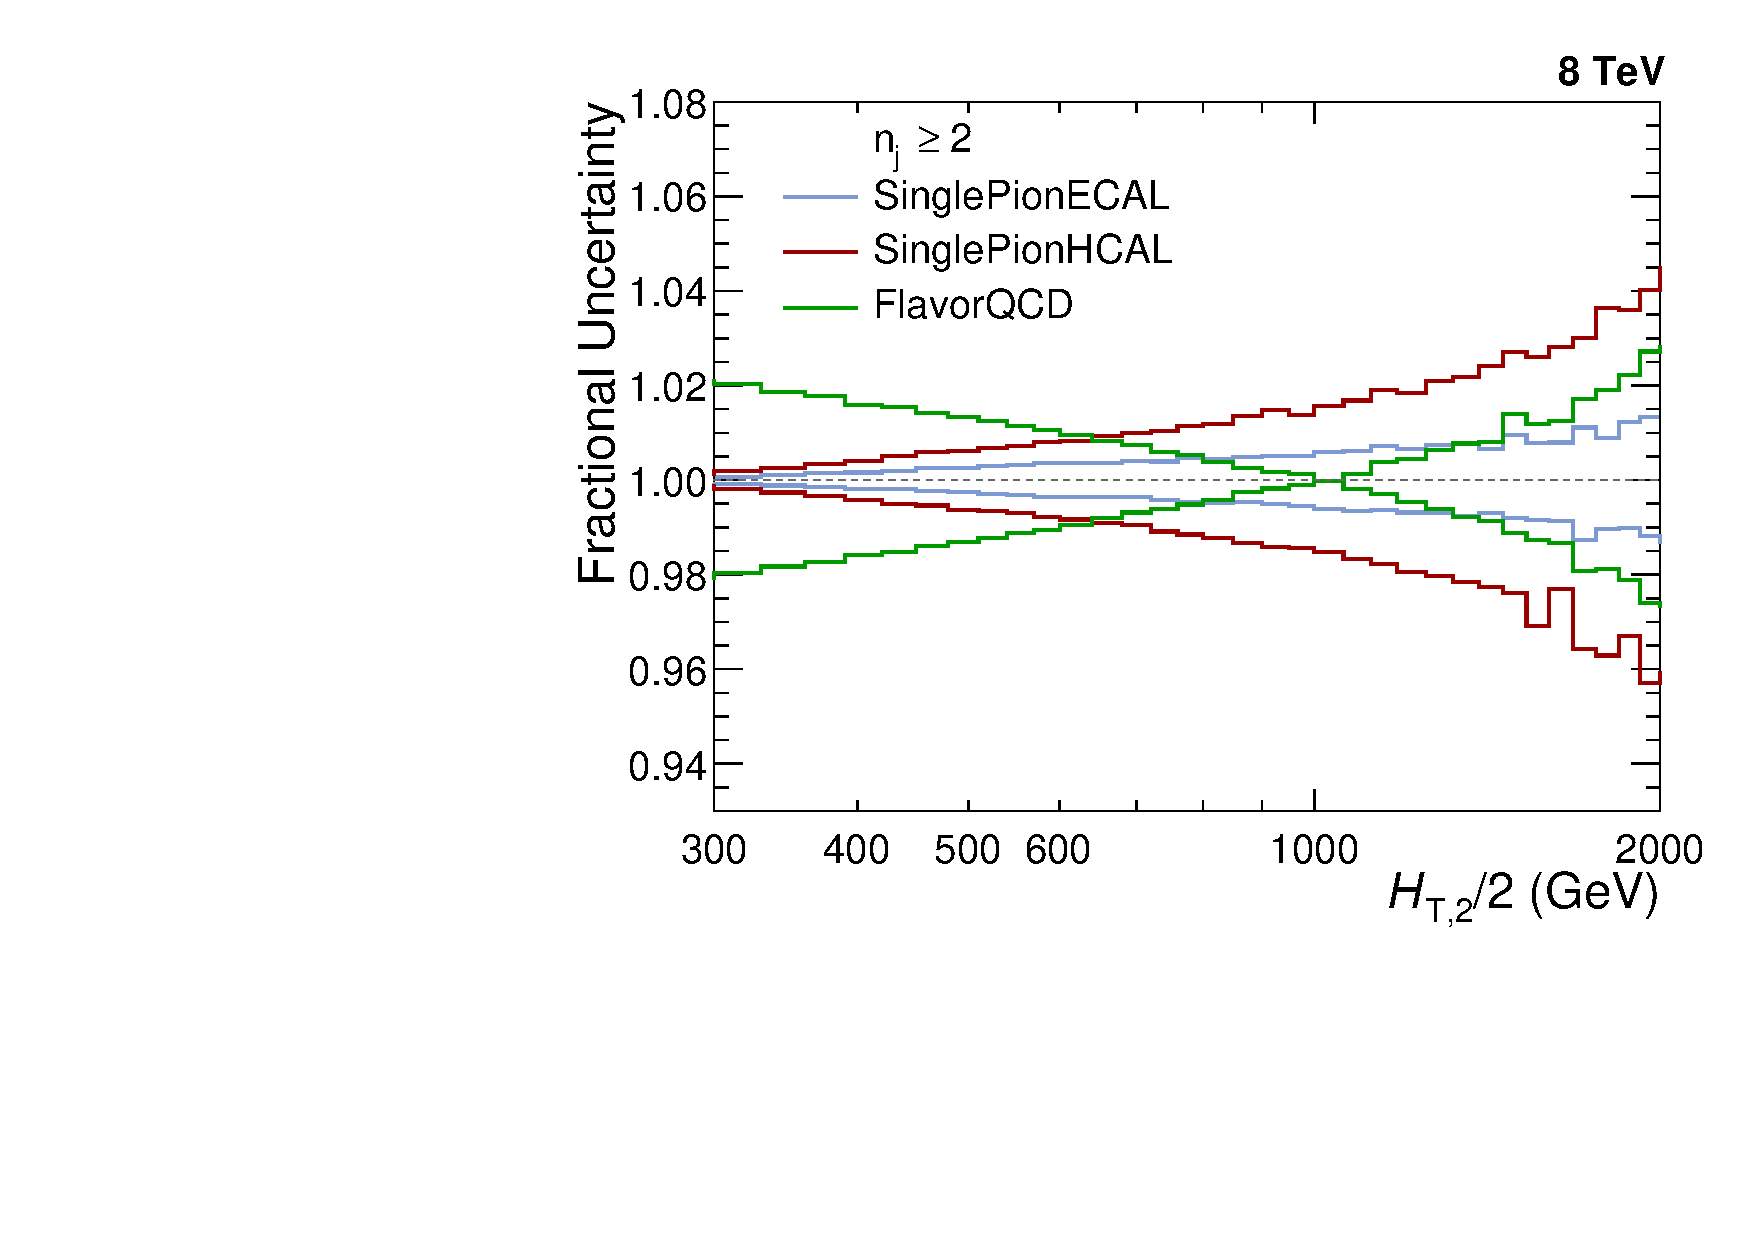
\includegraphics[width=0.51\textwidth]{/home/anter/Desktop/Thesis/Plots_HT_2_150/Single/MC_Macro_Plot_All_2_HT_2_Unc_Single_1.pdf}\\
\hspace*{-5mm}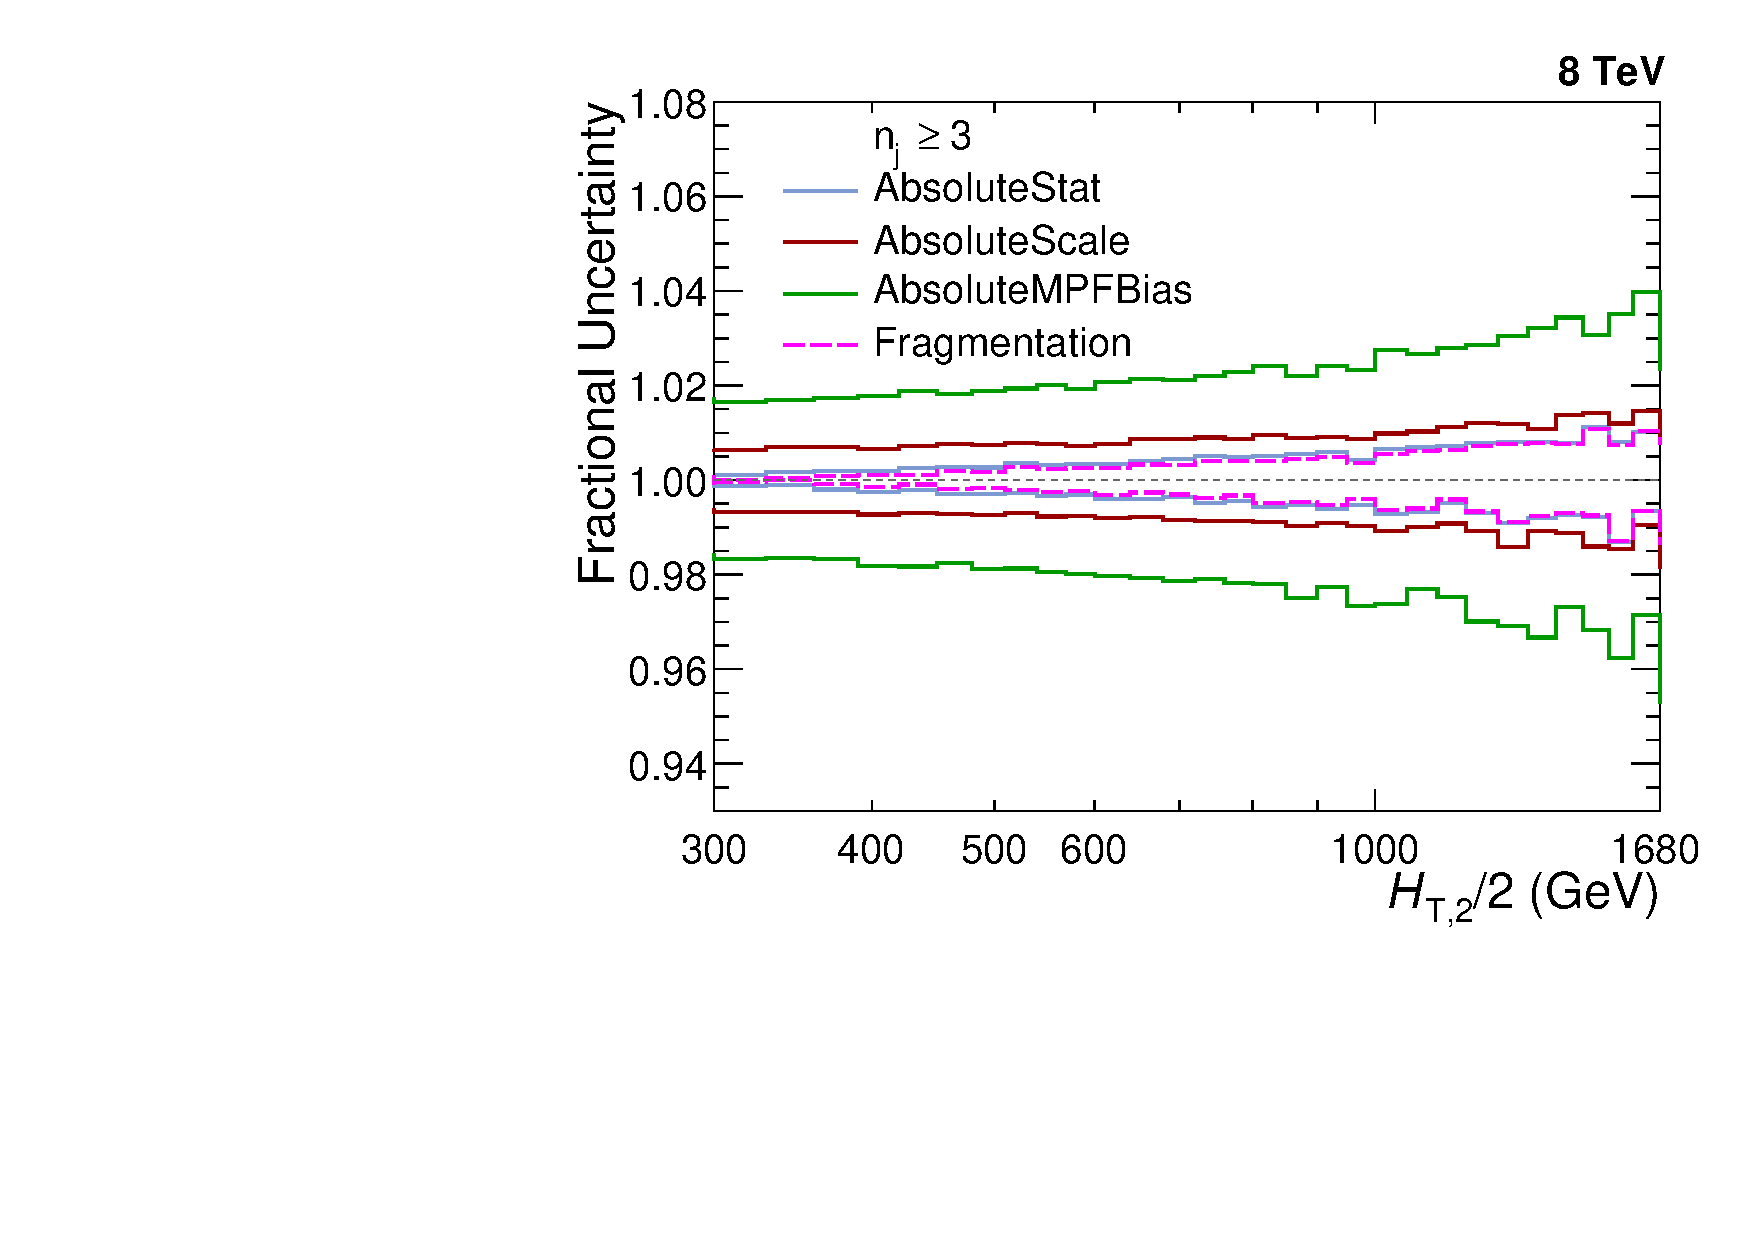
\includegraphics[width=0.51\textwidth]{/home/anter/Desktop/Thesis/Plots_HT_2_150/Single/MC_Macro_Plot_All_3_HT_2_Unc_Abs_1.pdf}%
~~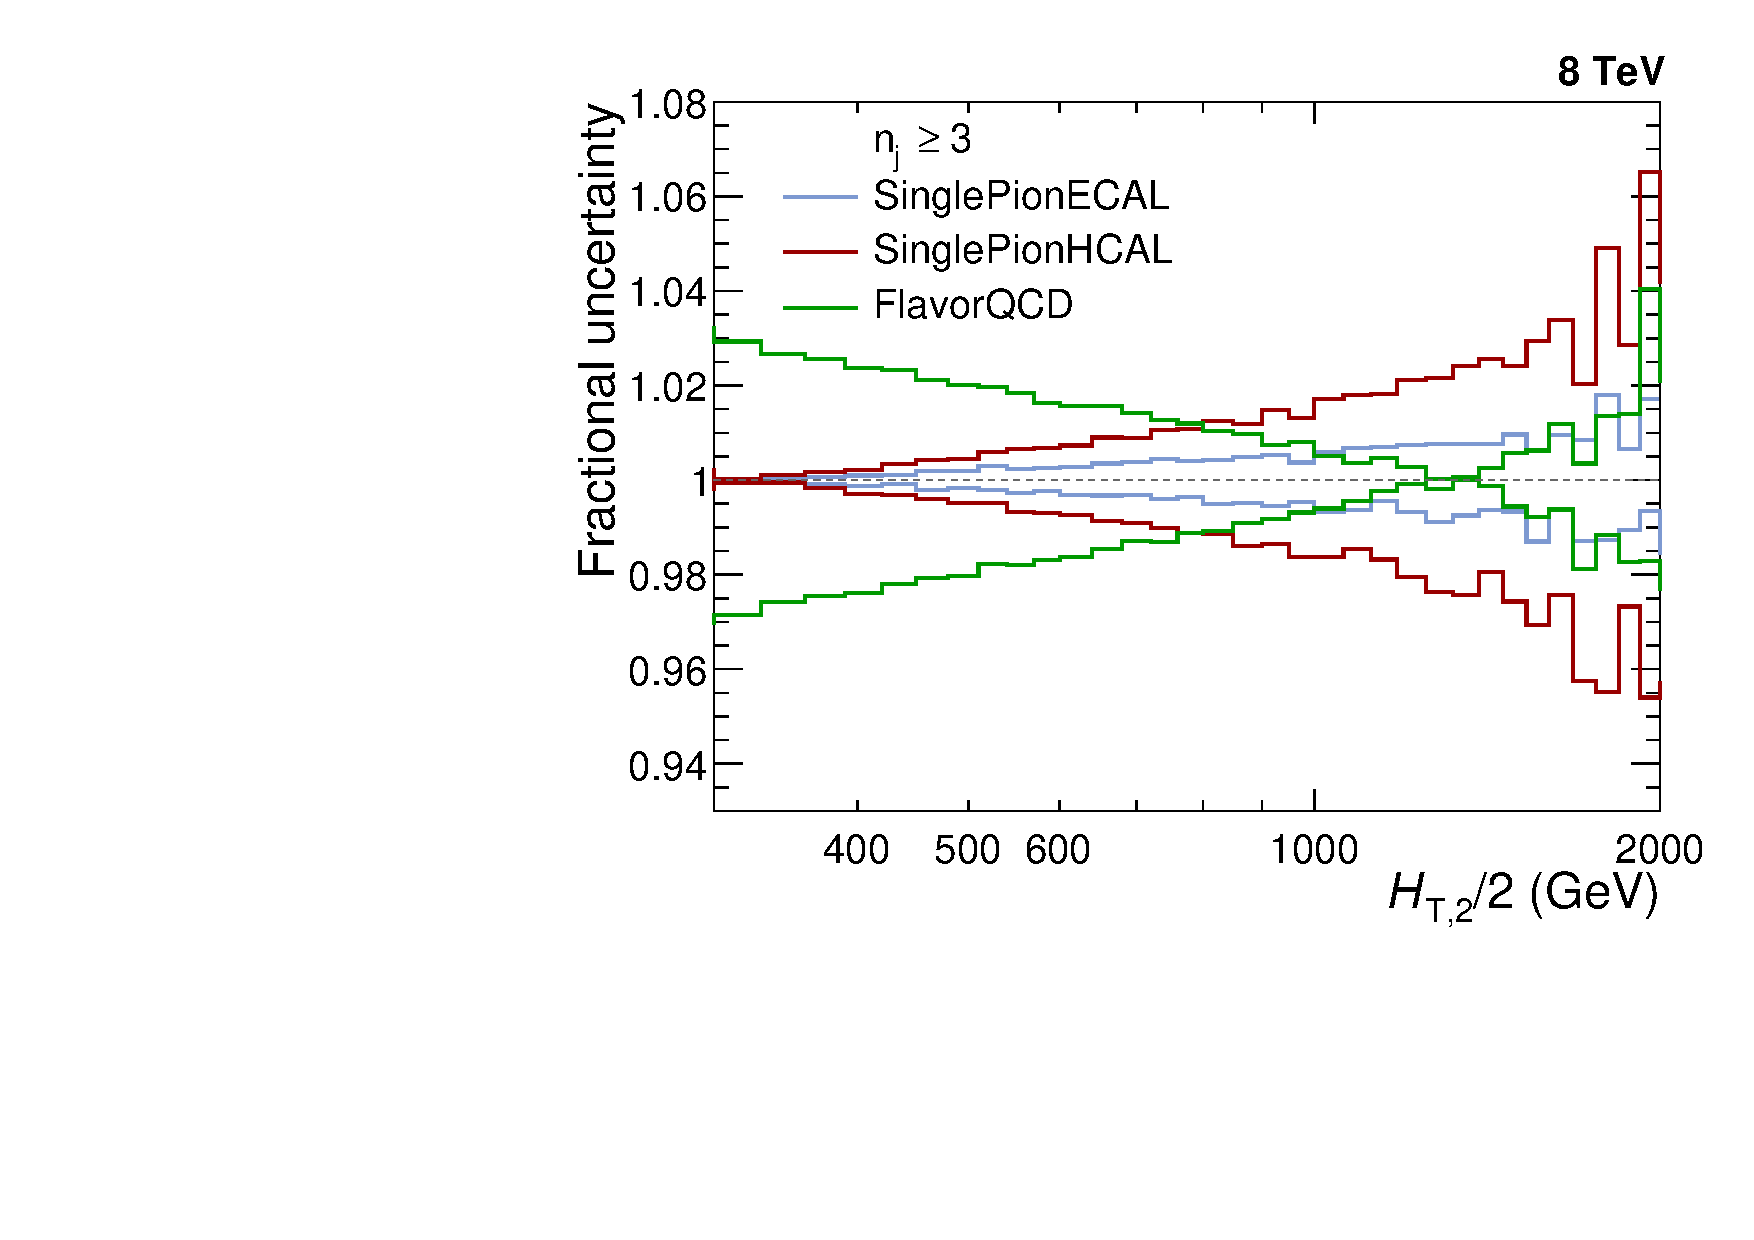
\includegraphics[width=0.51\textwidth]{/home/anter/Desktop/Thesis/Plots_HT_2_150/Single/MC_Macro_Plot_All_3_HT_2_Unc_Single_1.pdf}\\
\hspace*{-5mm}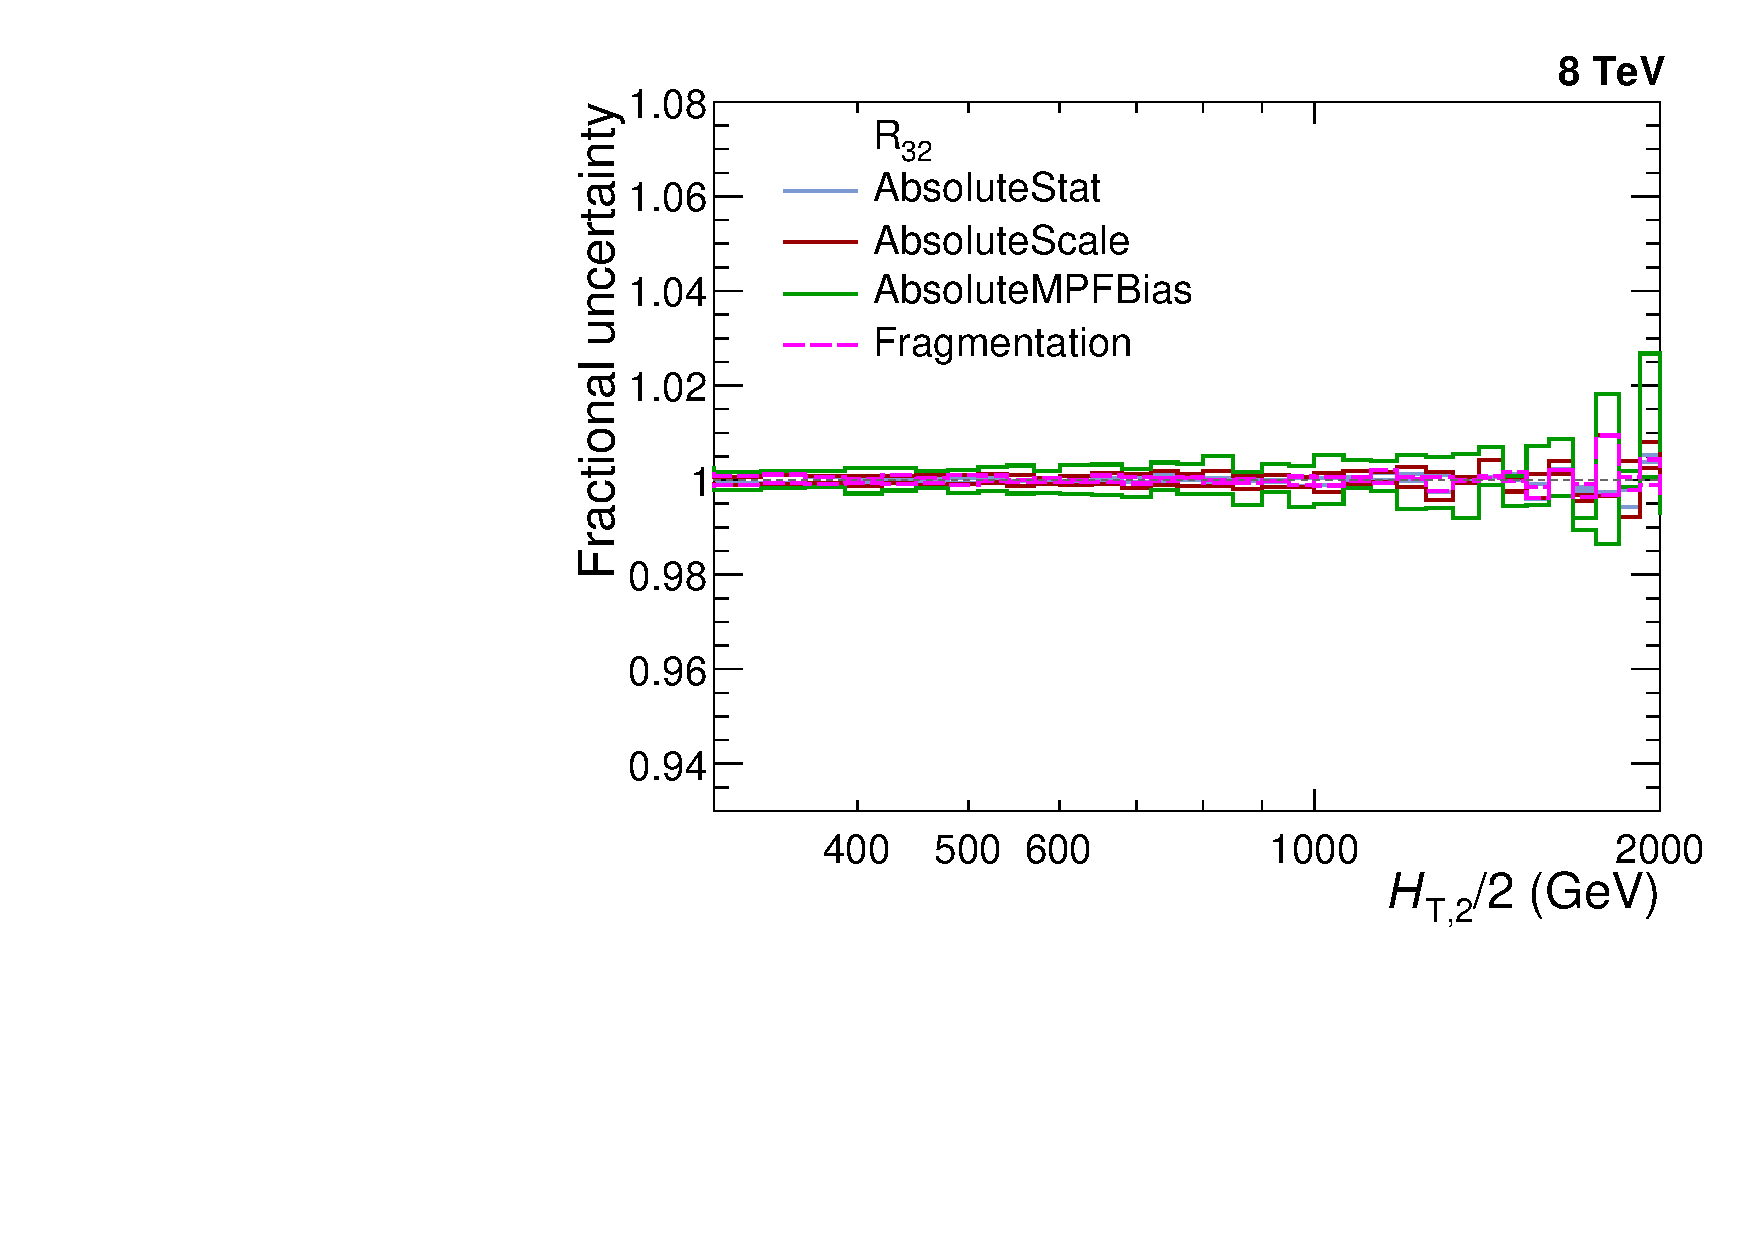
\includegraphics[width=0.51\textwidth]{/home/anter/Desktop/Thesis/Plots_HT_2_150/Single/MC_Macro_Plot_Ratio_32_HT_2_Unc_Abs_1.pdf}%
~~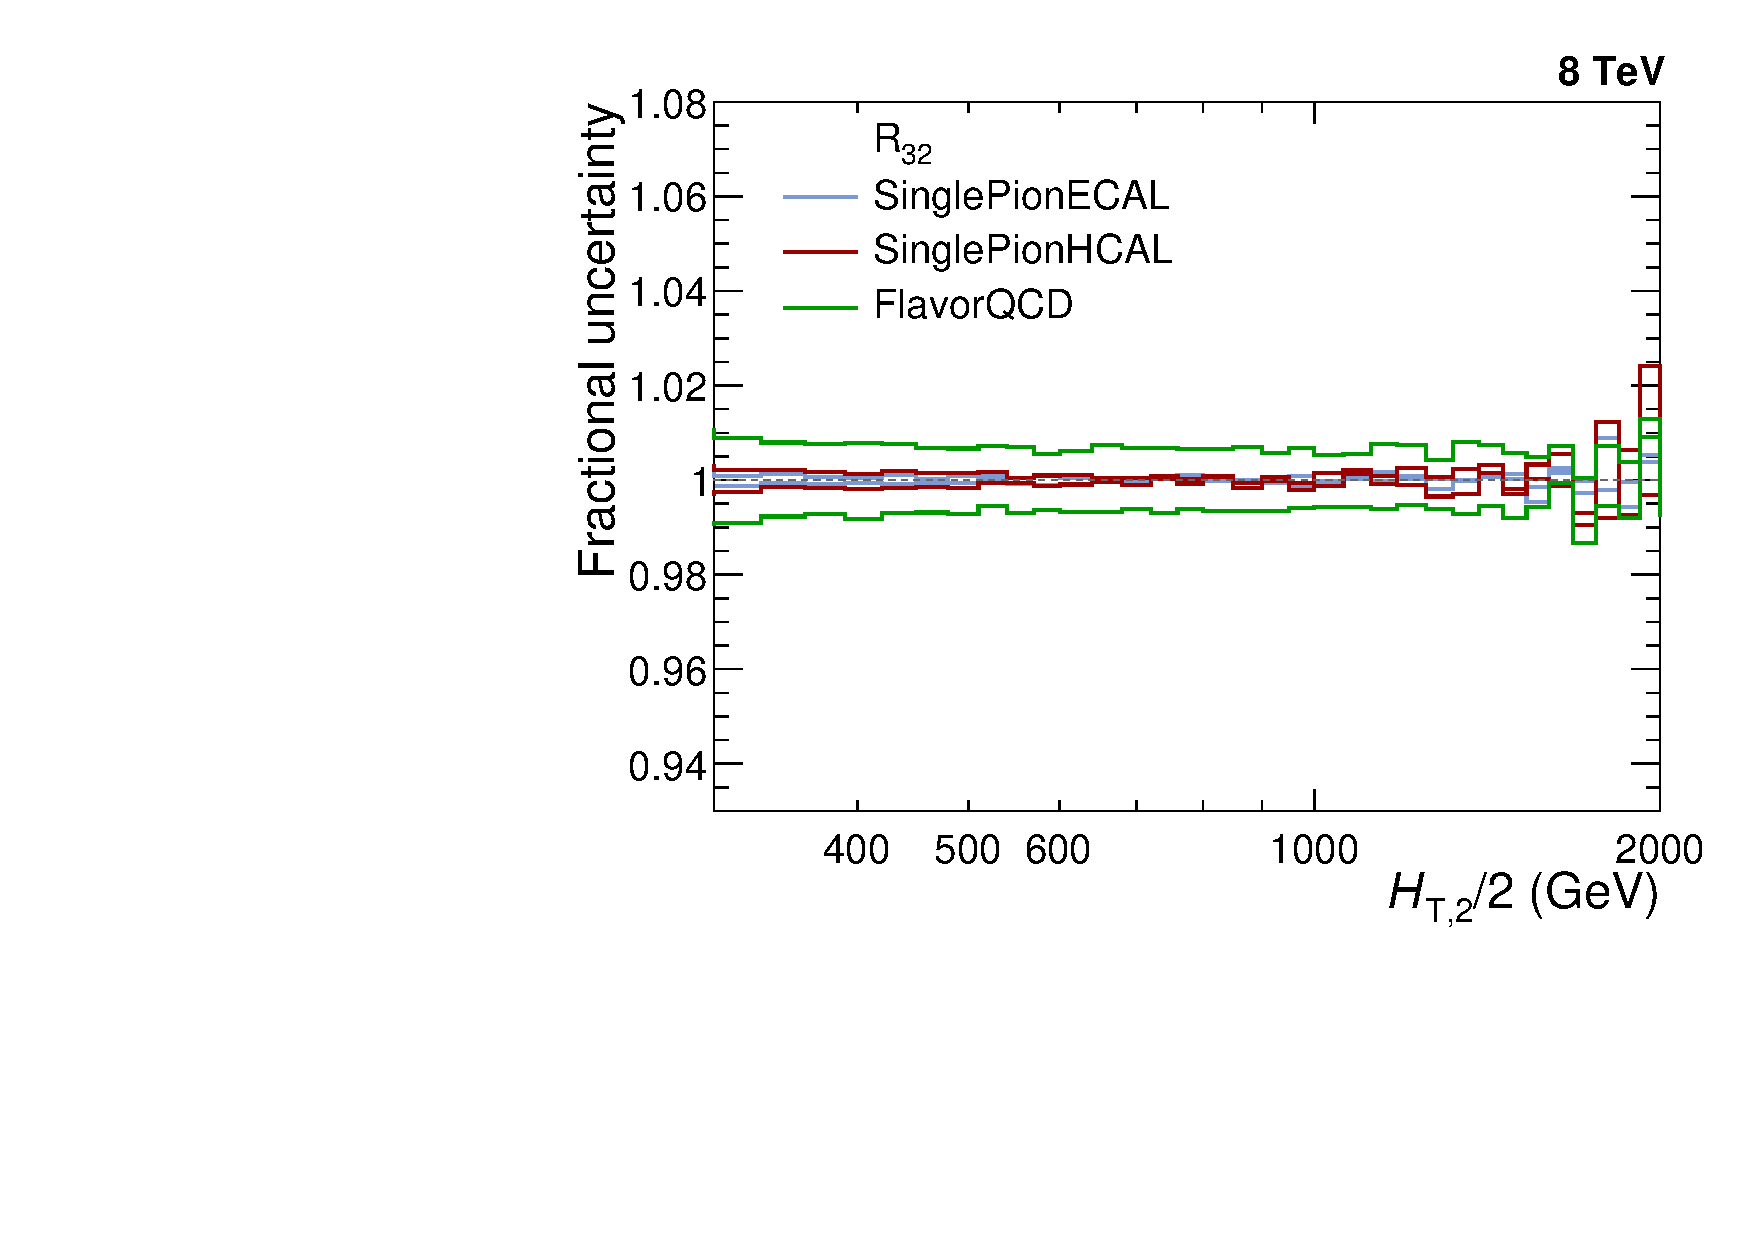
\includegraphics[width=0.51\textwidth]{/home/anter/Desktop/Thesis/Plots_HT_2_150/Single/MC_Macro_Plot_Ratio_32_HT_2_Unc_Single_1.pdf}\\
\caption{The relative size of the jet energy correction (JEC) uncertainties for individual sources are shown for inclusive 2-jet (top) and 3-jet events cross sections (middle); and cross section ratio \ratio (bottom). On left, JEC uncertainties are evaluated from \textcolor{blue2}{AbsoluteStat}, \textcolor{red}{AbsoluteScale}, \textcolor{green}{AbsoluteMPFBias} and \textcolor{pink2}{Fragmentation} sources whereas on right, these are evaluated from \textcolor{blue2}{SinglePionECAL}, \textcolor{red}{SinglePionHCAL} and \textcolor{green}{FlavorQCD} sources.}
\label{fig:jes1}
%\end{center}
\end{figure}

\begin{figure}[!hbtp]
%\begin{center}
\hspace*{-5mm}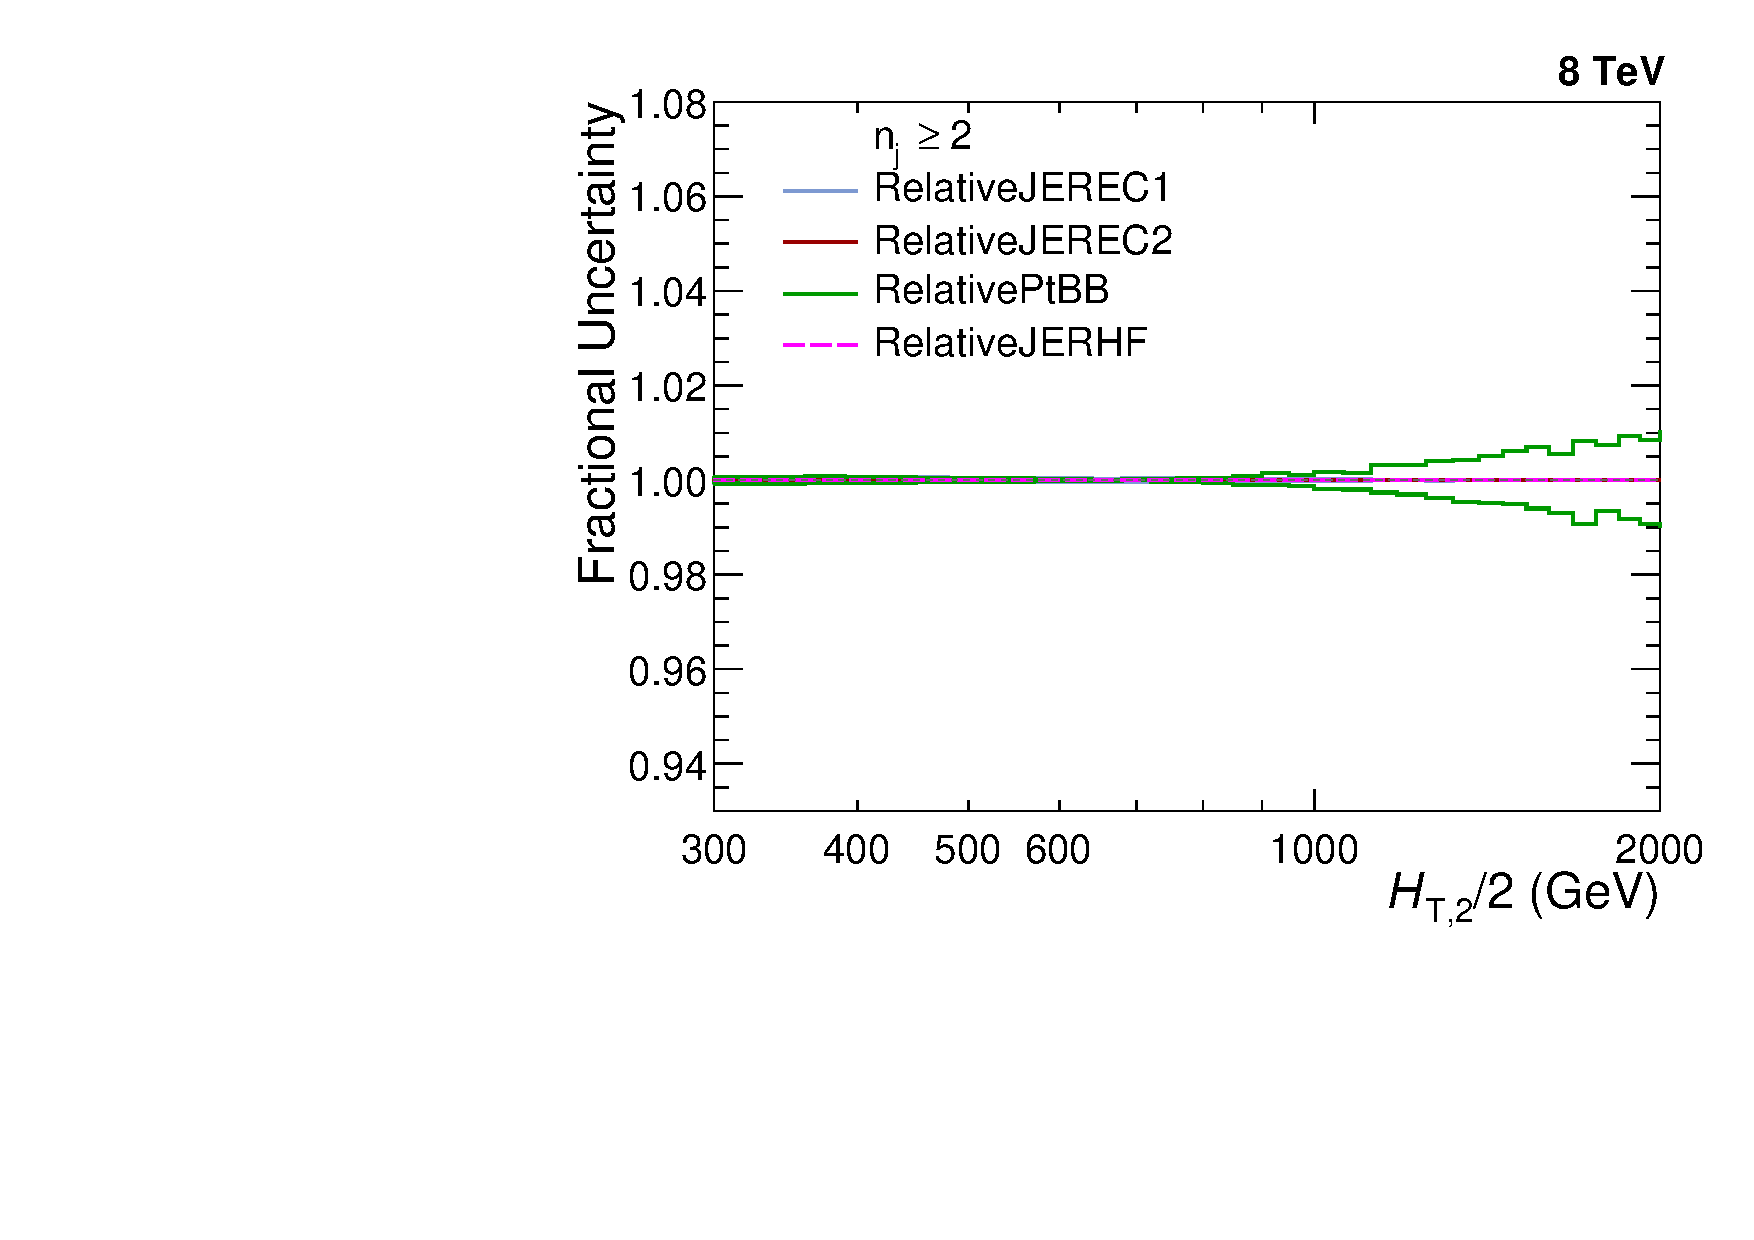
\includegraphics[width=0.51\textwidth]{/home/anter/Desktop/Thesis/Plots_HT_2_150/Single/MC_Macro_Plot_All_2_HT_2_Unc_Relative_1.pdf}%
~~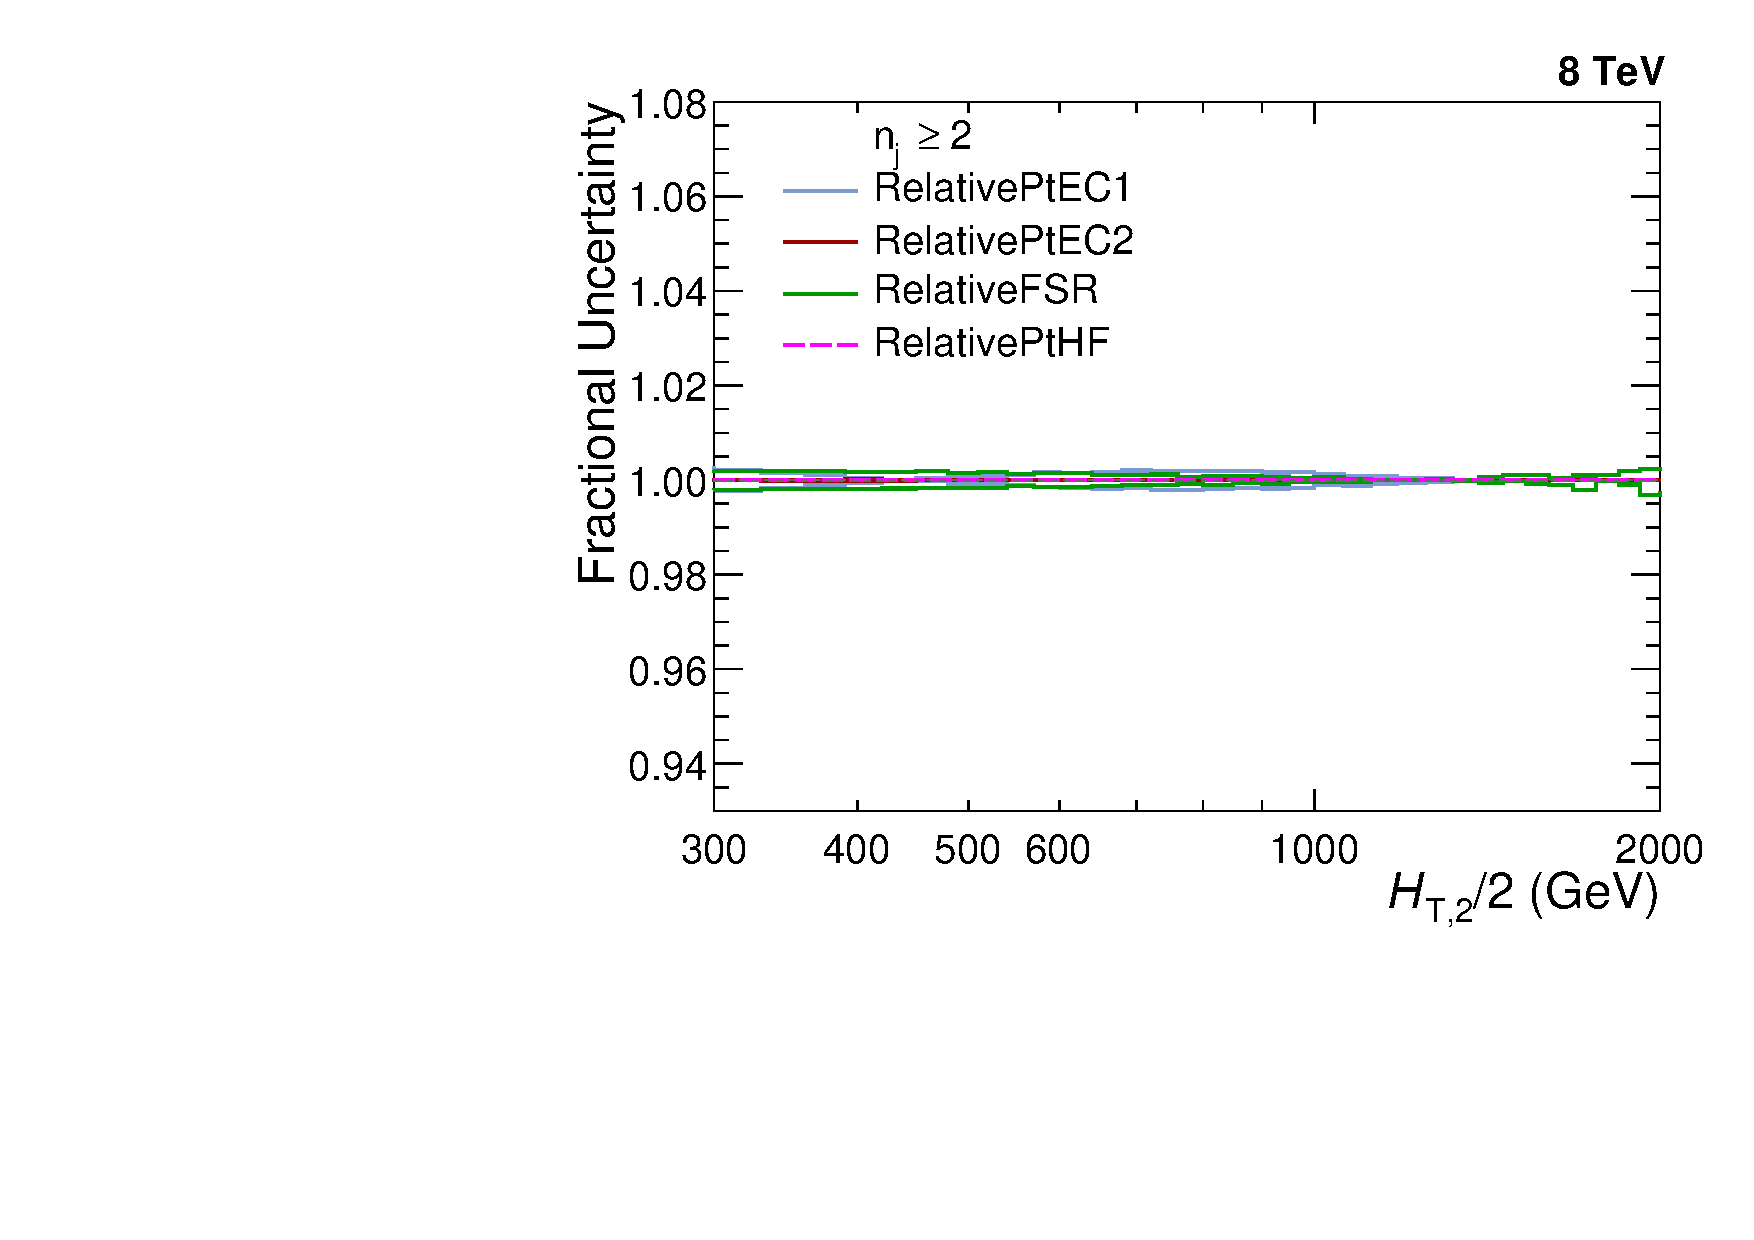
\includegraphics[width=0.51\textwidth]{/home/anter/Desktop/Thesis/Plots_HT_2_150/Single/MC_Macro_Plot_All_2_HT_2_Unc_Relative_2.pdf}\\
\hspace*{-5mm}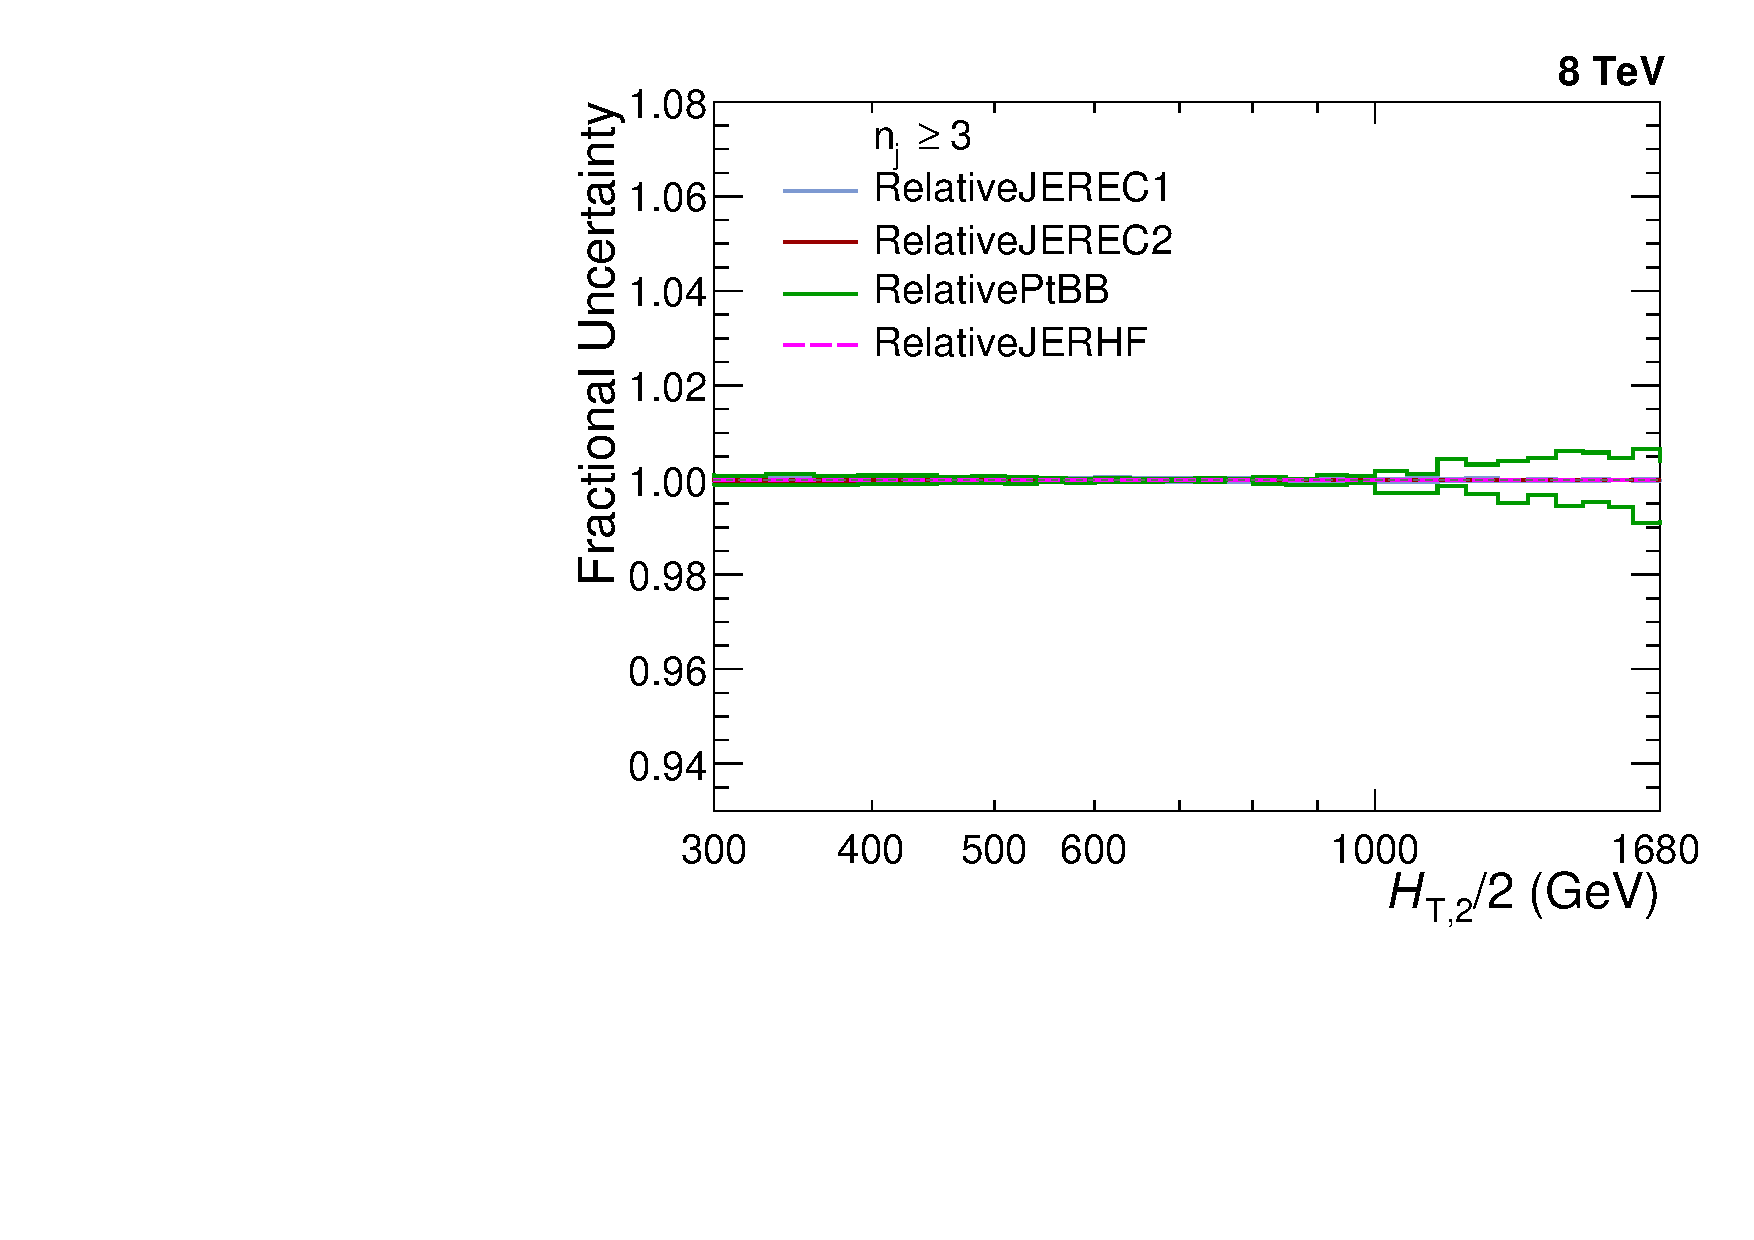
\includegraphics[width=0.51\textwidth]{/home/anter/Desktop/Thesis/Plots_HT_2_150/Single/MC_Macro_Plot_All_3_HT_2_Unc_Relative_1.pdf}%
~~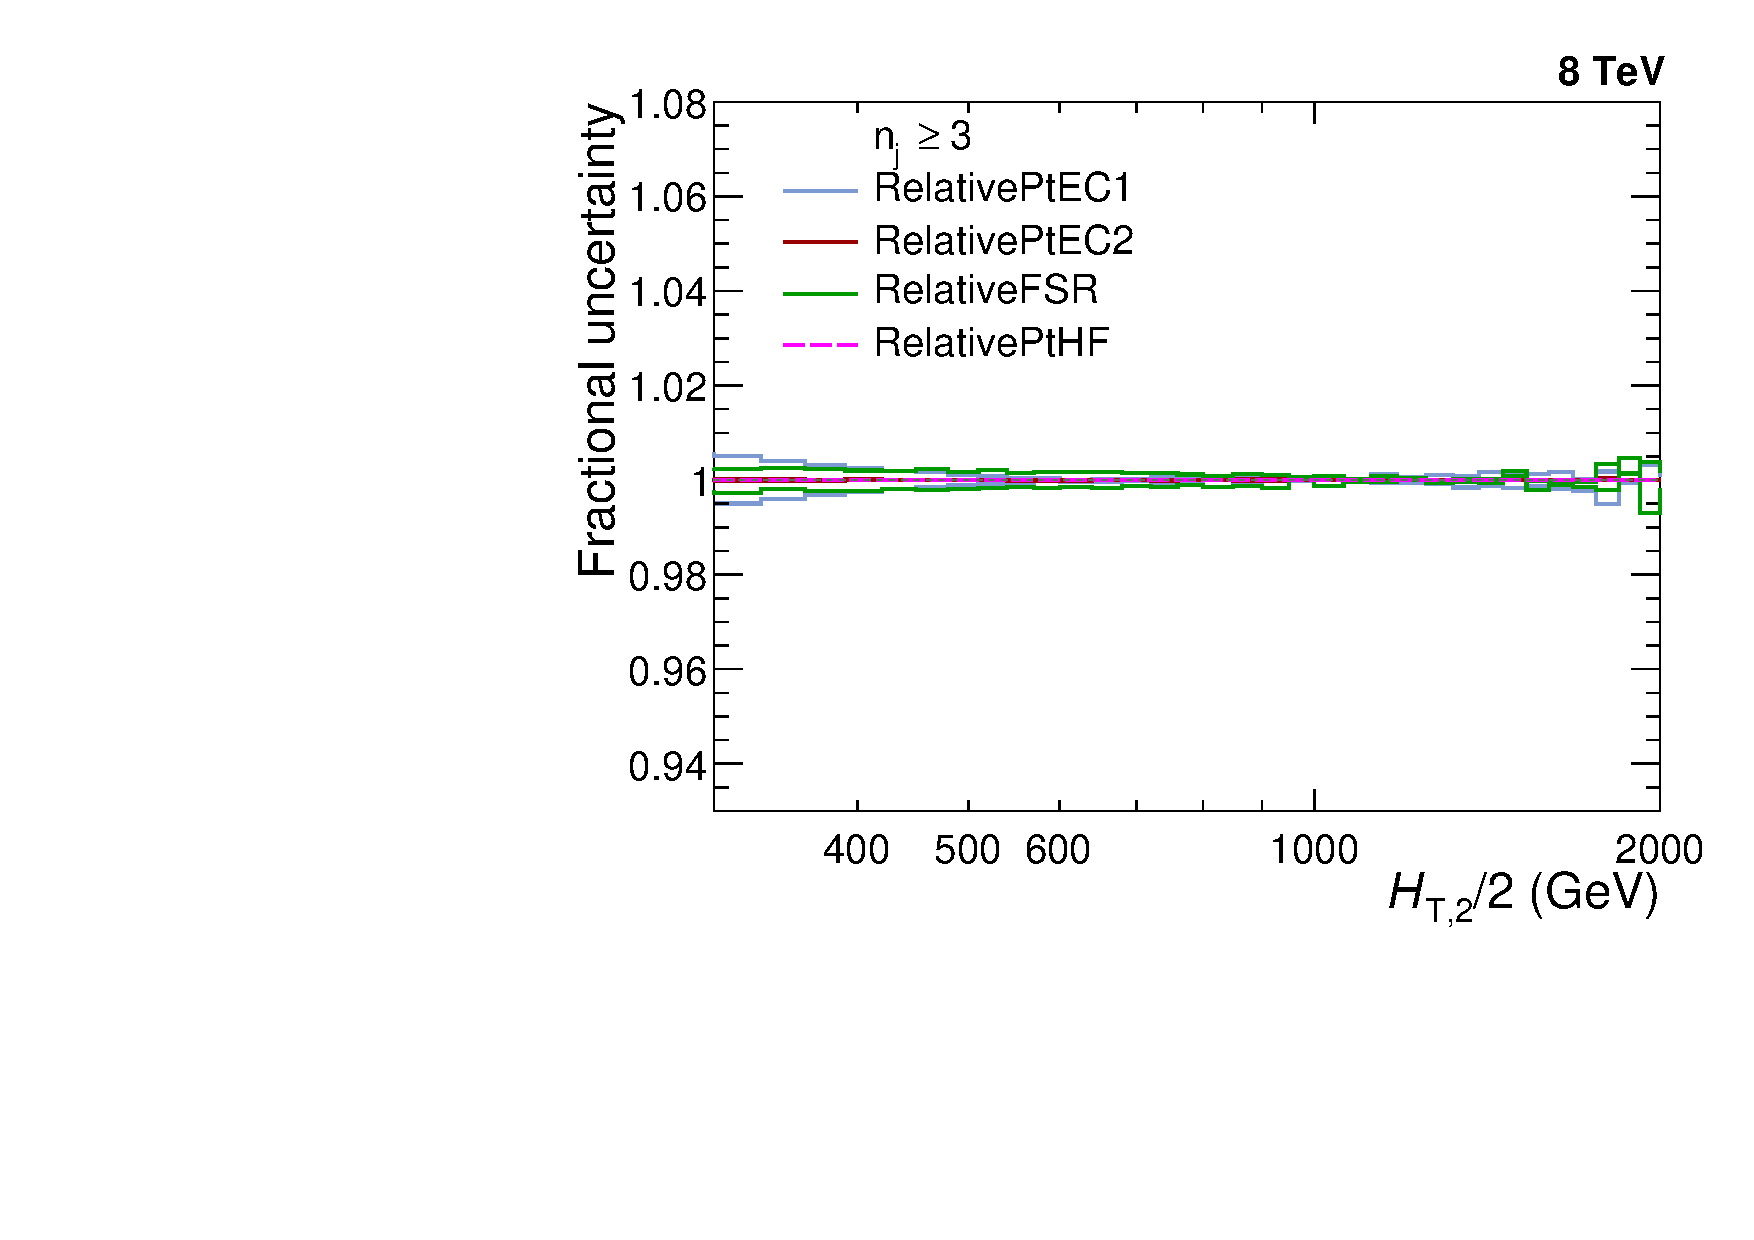
\includegraphics[width=0.51\textwidth]{/home/anter/Desktop/Thesis/Plots_HT_2_150/Single/MC_Macro_Plot_All_3_HT_2_Unc_Relative_2.pdf}\\
\hspace*{-5mm}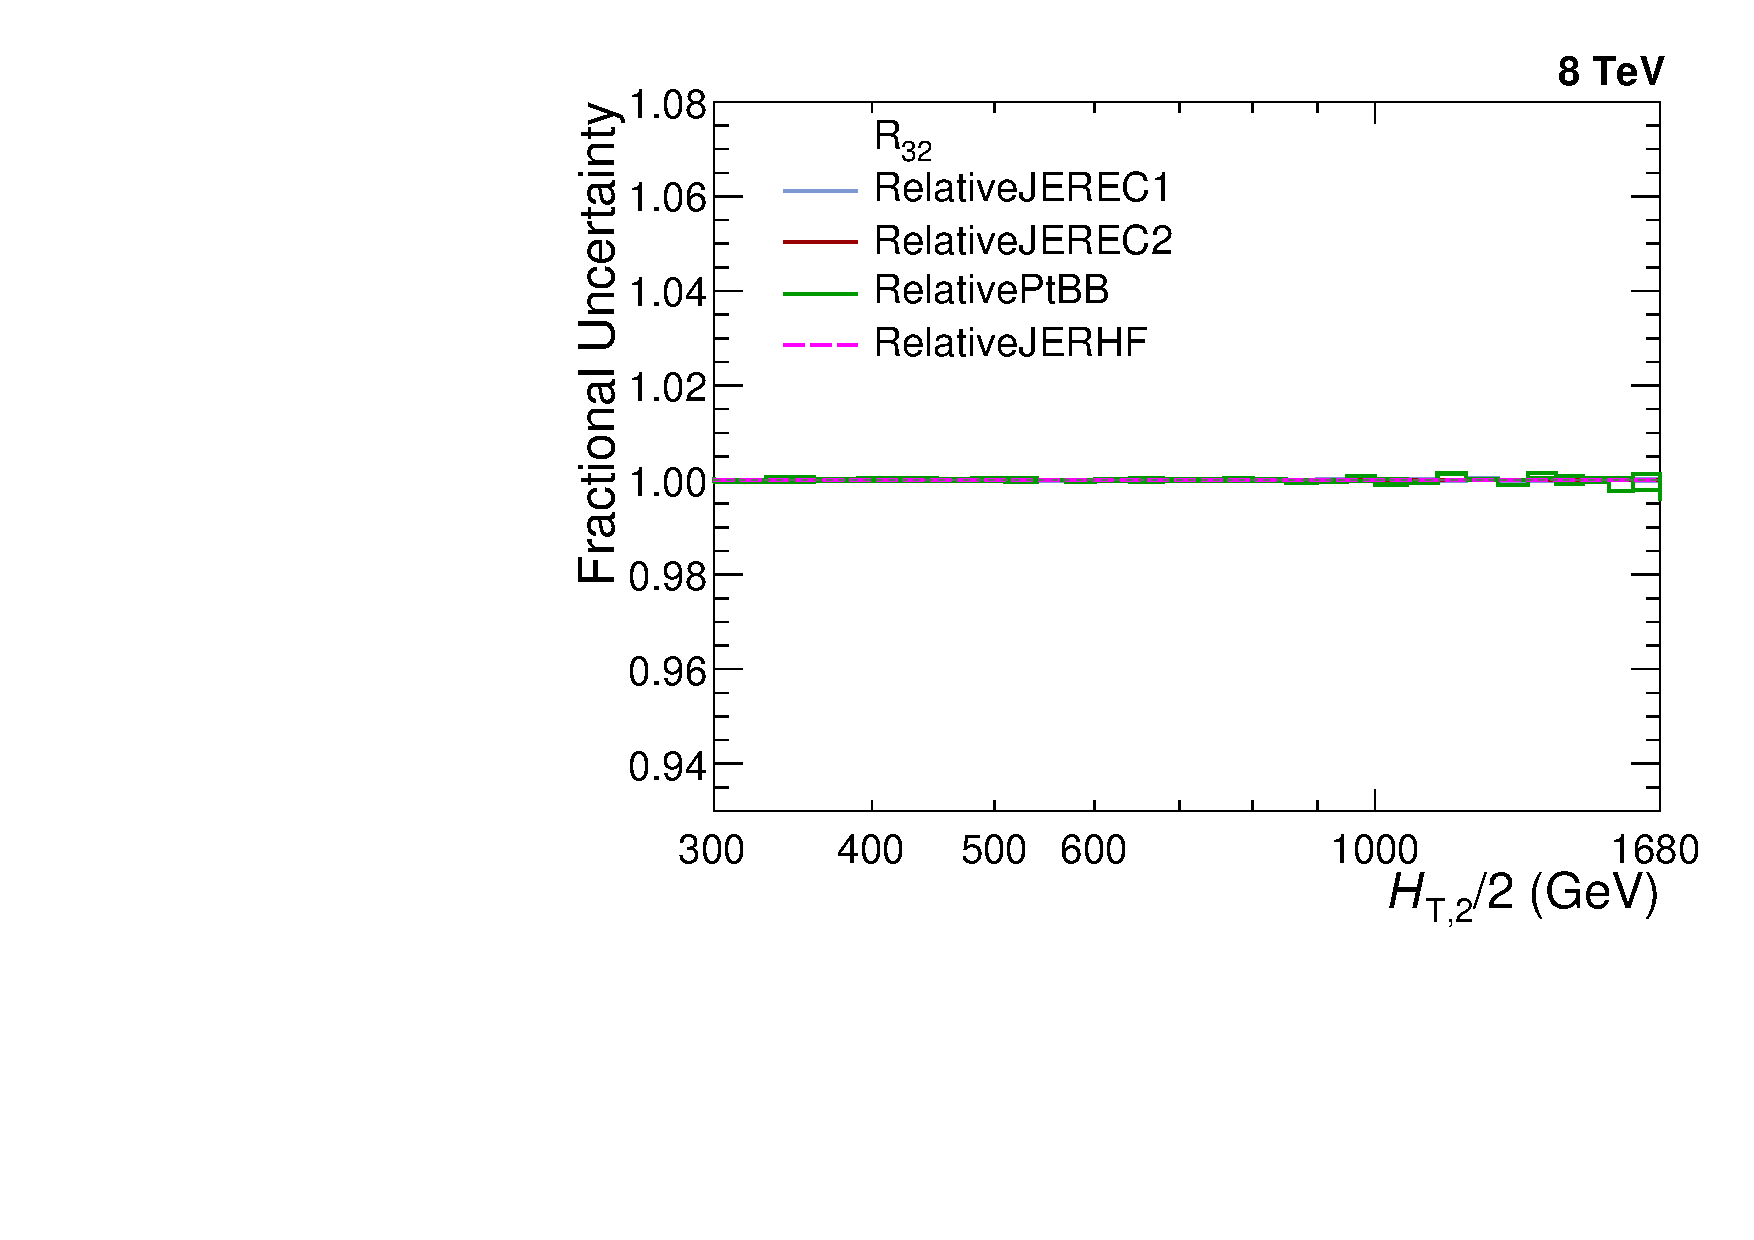
\includegraphics[width=0.51\textwidth]{/home/anter/Desktop/Thesis/Plots_HT_2_150/Single/MC_Macro_Plot_Ratio_32_HT_2_Unc_Relative_1.pdf}%
~~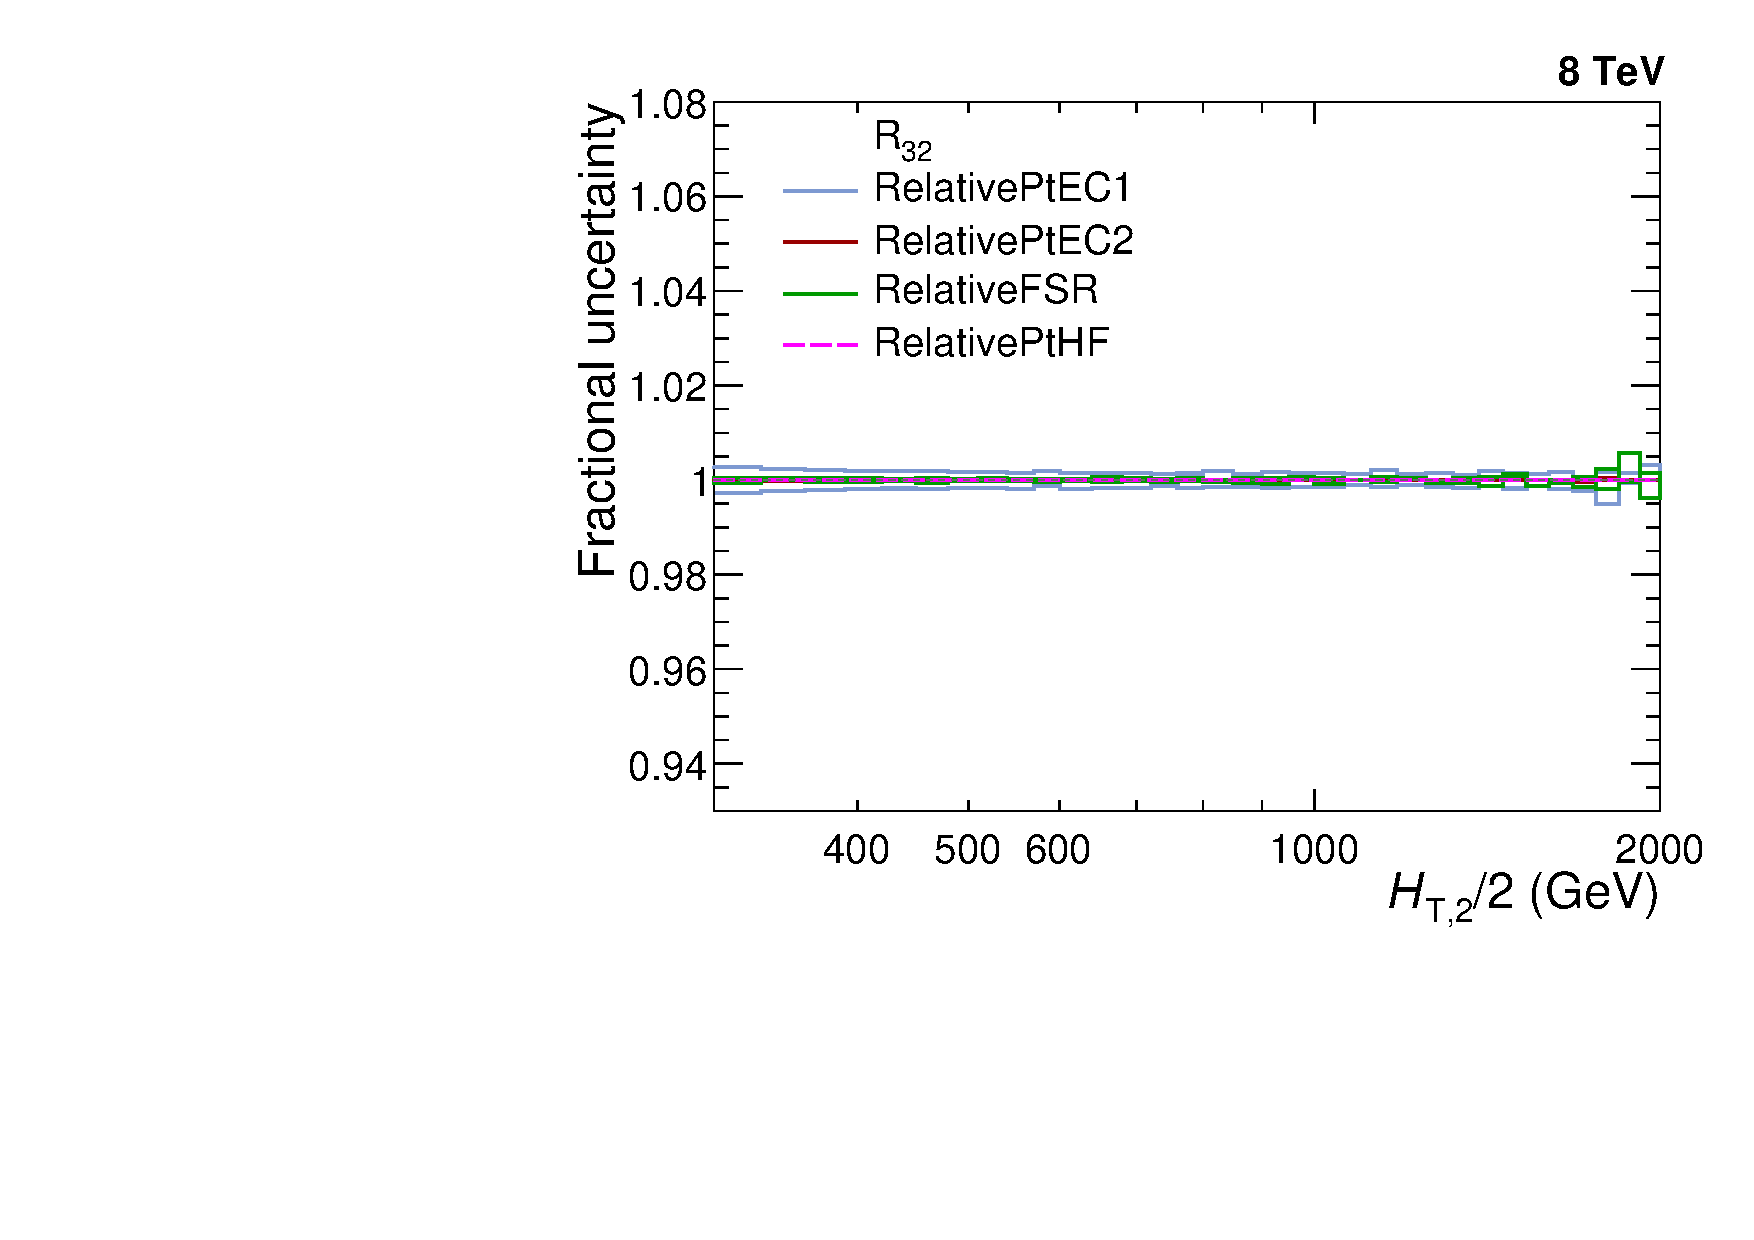
\includegraphics[width=0.51\textwidth]{/home/anter/Desktop/Thesis/Plots_HT_2_150/Single/MC_Macro_Plot_Ratio_32_HT_2_Unc_Relative_2.pdf}\\
\caption{The relative size of the jet energy correction (JEC) uncertainties for individual sources are shown for inclusive 2-jet (top) and 3-jet events cross sections (middle); and cross section ratio \ratio (bottom). On left, JEC uncertainties are evaluated from \textcolor{blue2}{RelativeJEREC1}, \textcolor{red}{RelativeJEREC2}, \textcolor{green}{RelativePtBB} and \textcolor{pink2}{RelativeJERHF} sources whereas on right, these are evaluated from \textcolor{blue2}{RelativePtEC1}, \textcolor{red}{RelativePtEC2}, \textcolor{green}{RelativePFSR} and \textcolor{pink2}{RelativePtHF} sources.}
\label{fig:jes2}
%\end{center}
\end{figure}

\begin{figure}[!hbtp]
%\begin{center}
\hspace*{-5mm}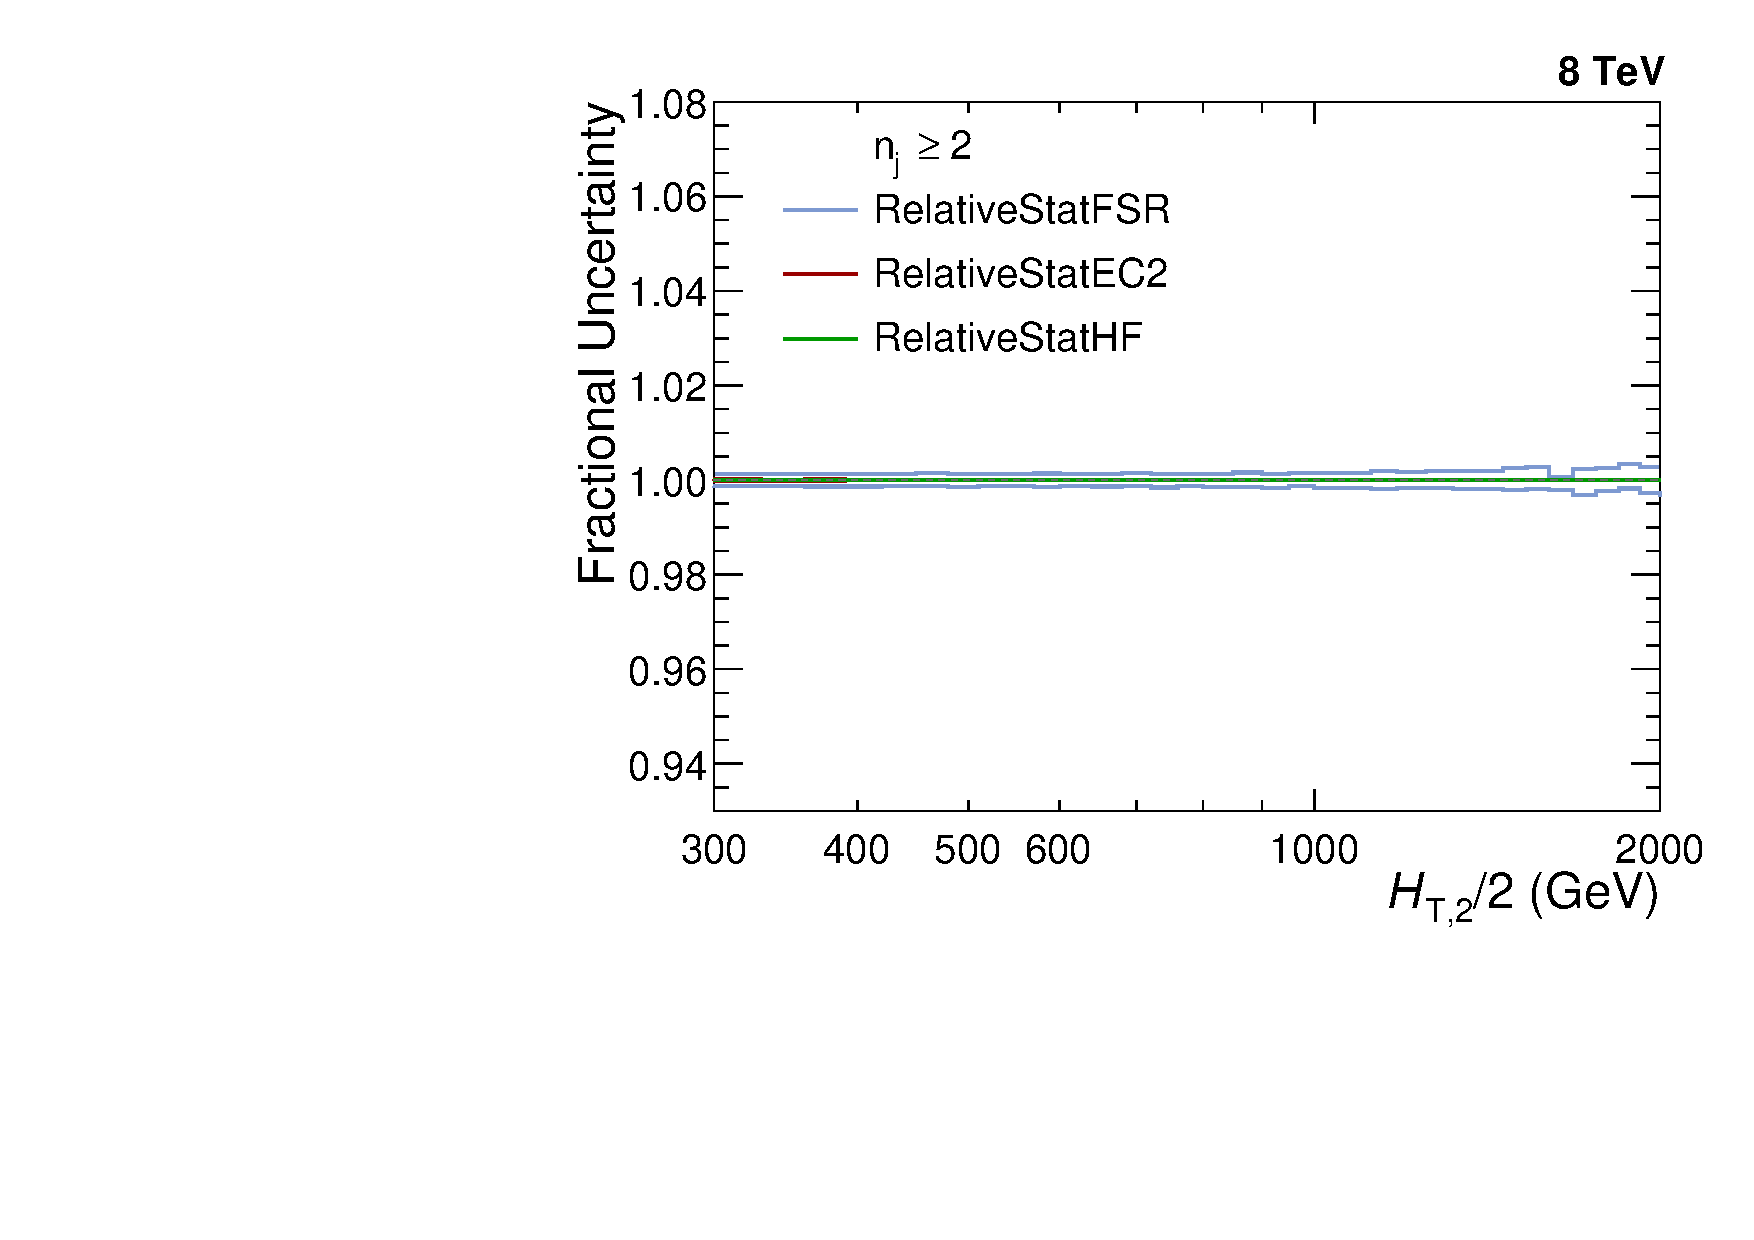
\includegraphics[width=0.51\textwidth]{/home/anter/Desktop/Thesis/Plots_HT_2_150/Single/MC_Macro_Plot_All_2_HT_2_Unc_RelativeStat_1.pdf}%
~~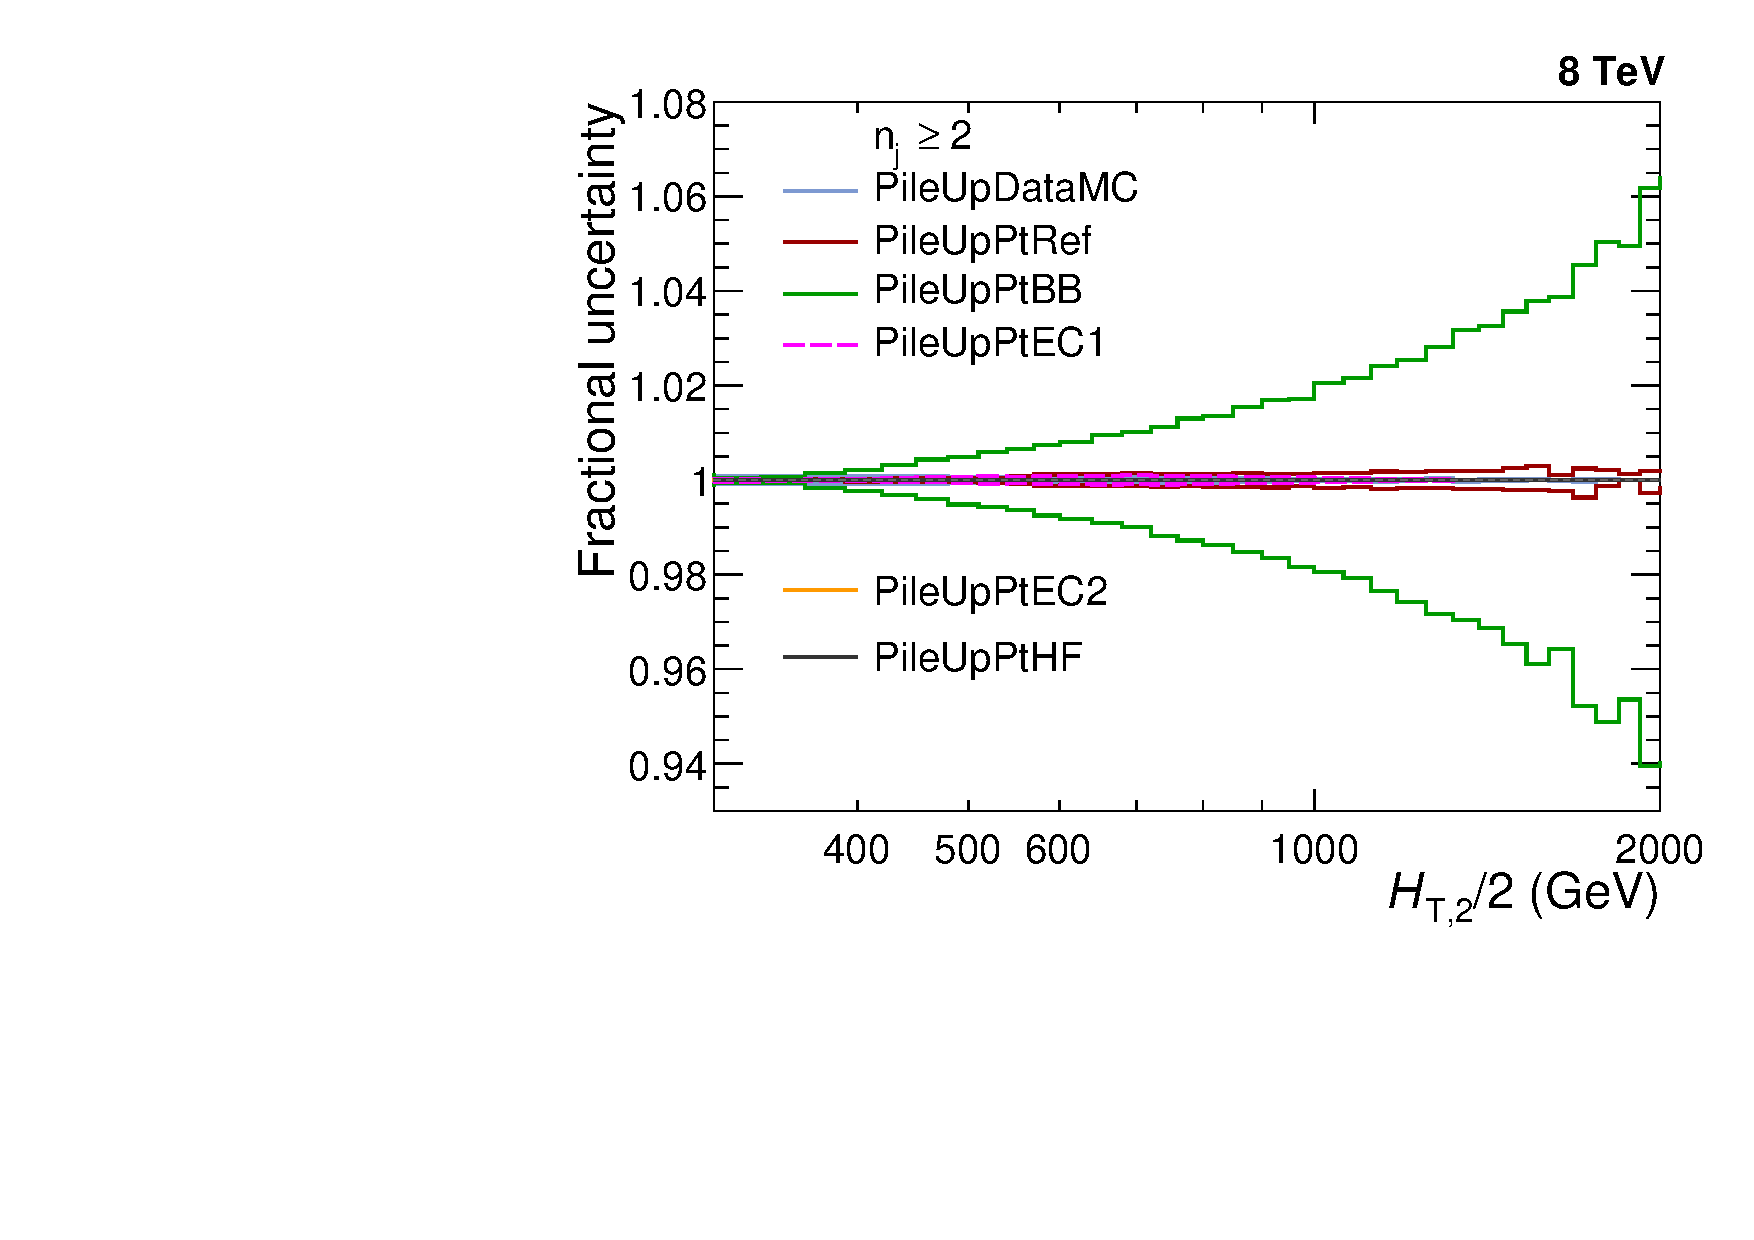
\includegraphics[width=0.51\textwidth]{/home/anter/Desktop/Thesis/Plots_HT_2_150/Single/MC_Macro_Plot_All_2_HT_2_Unc_Pileup_1.pdf}\\
\hspace*{-5mm}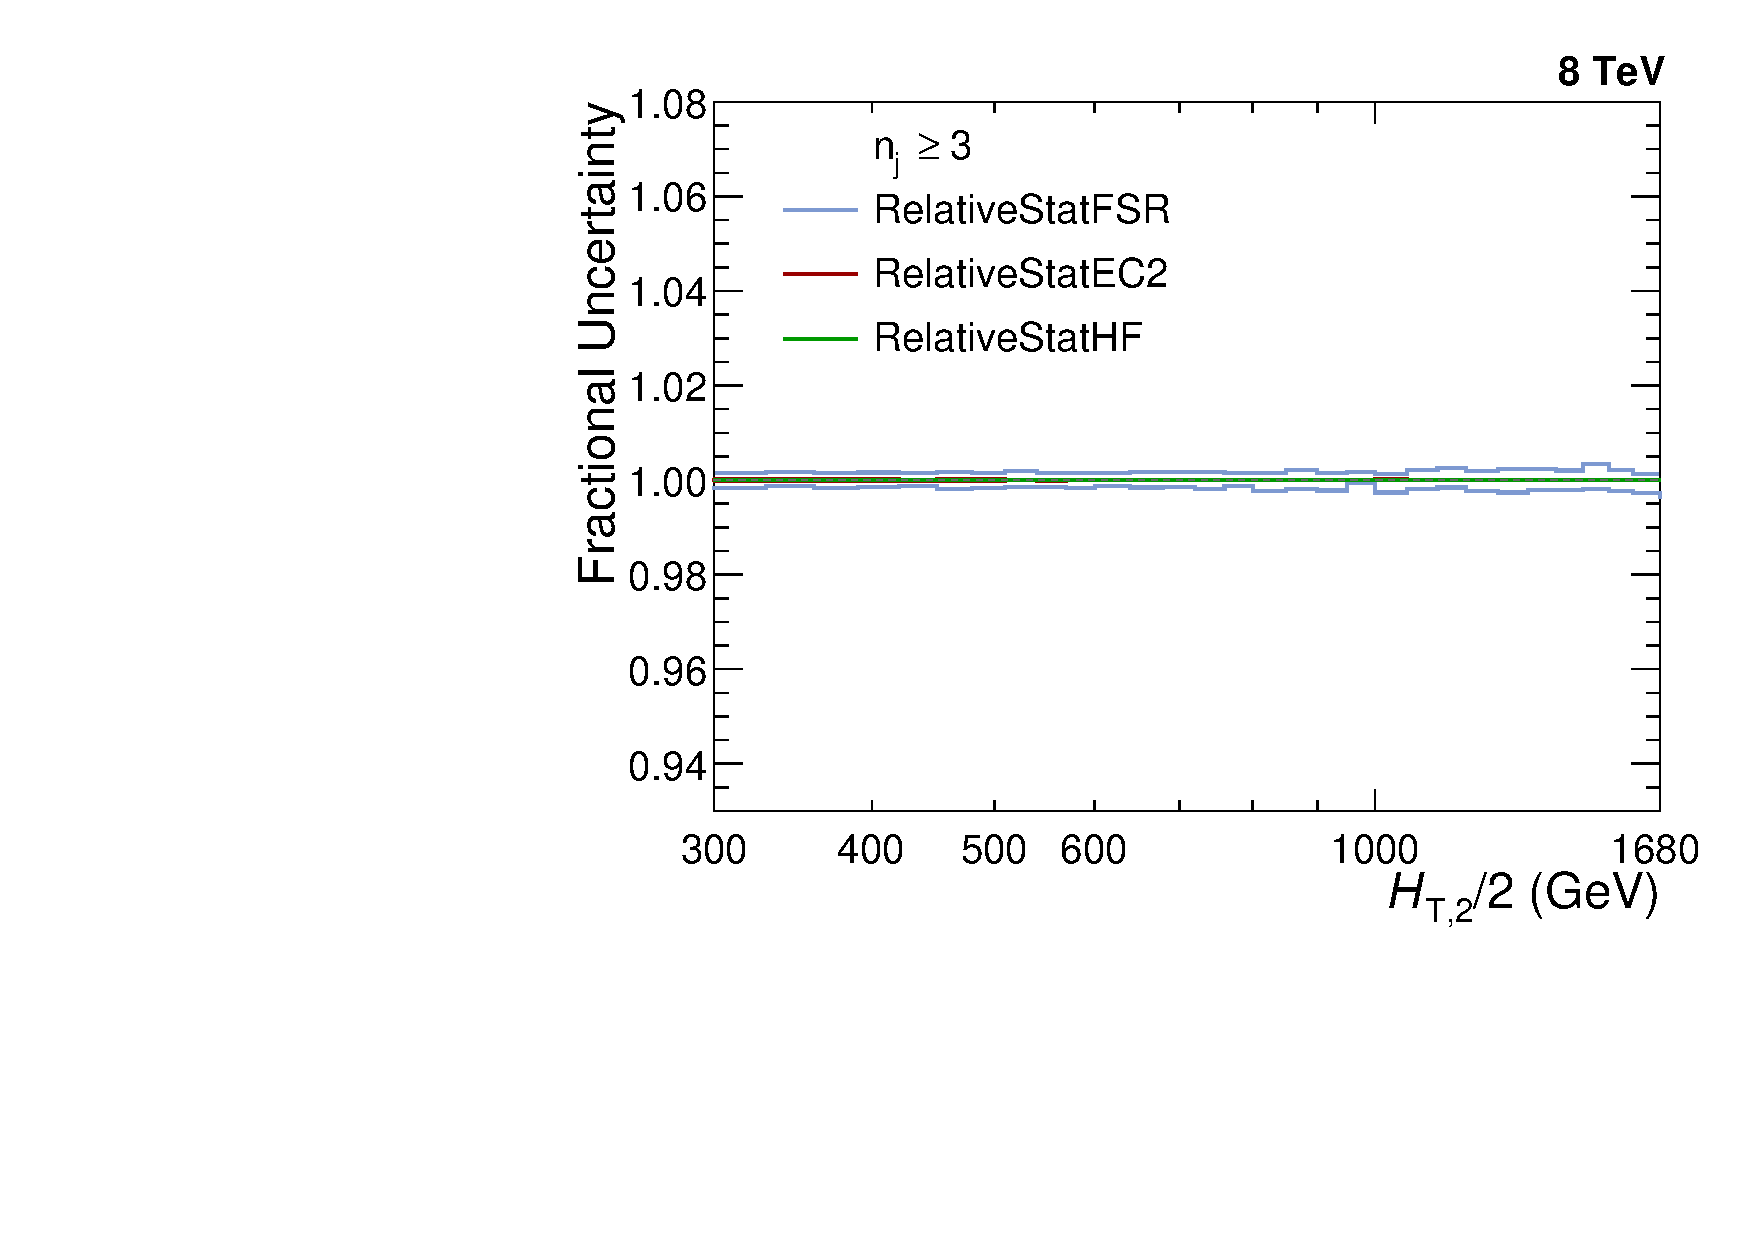
\includegraphics[width=0.51\textwidth]{/home/anter/Desktop/Thesis/Plots_HT_2_150/Single/MC_Macro_Plot_All_3_HT_2_Unc_RelativeStat_1.pdf}%
~~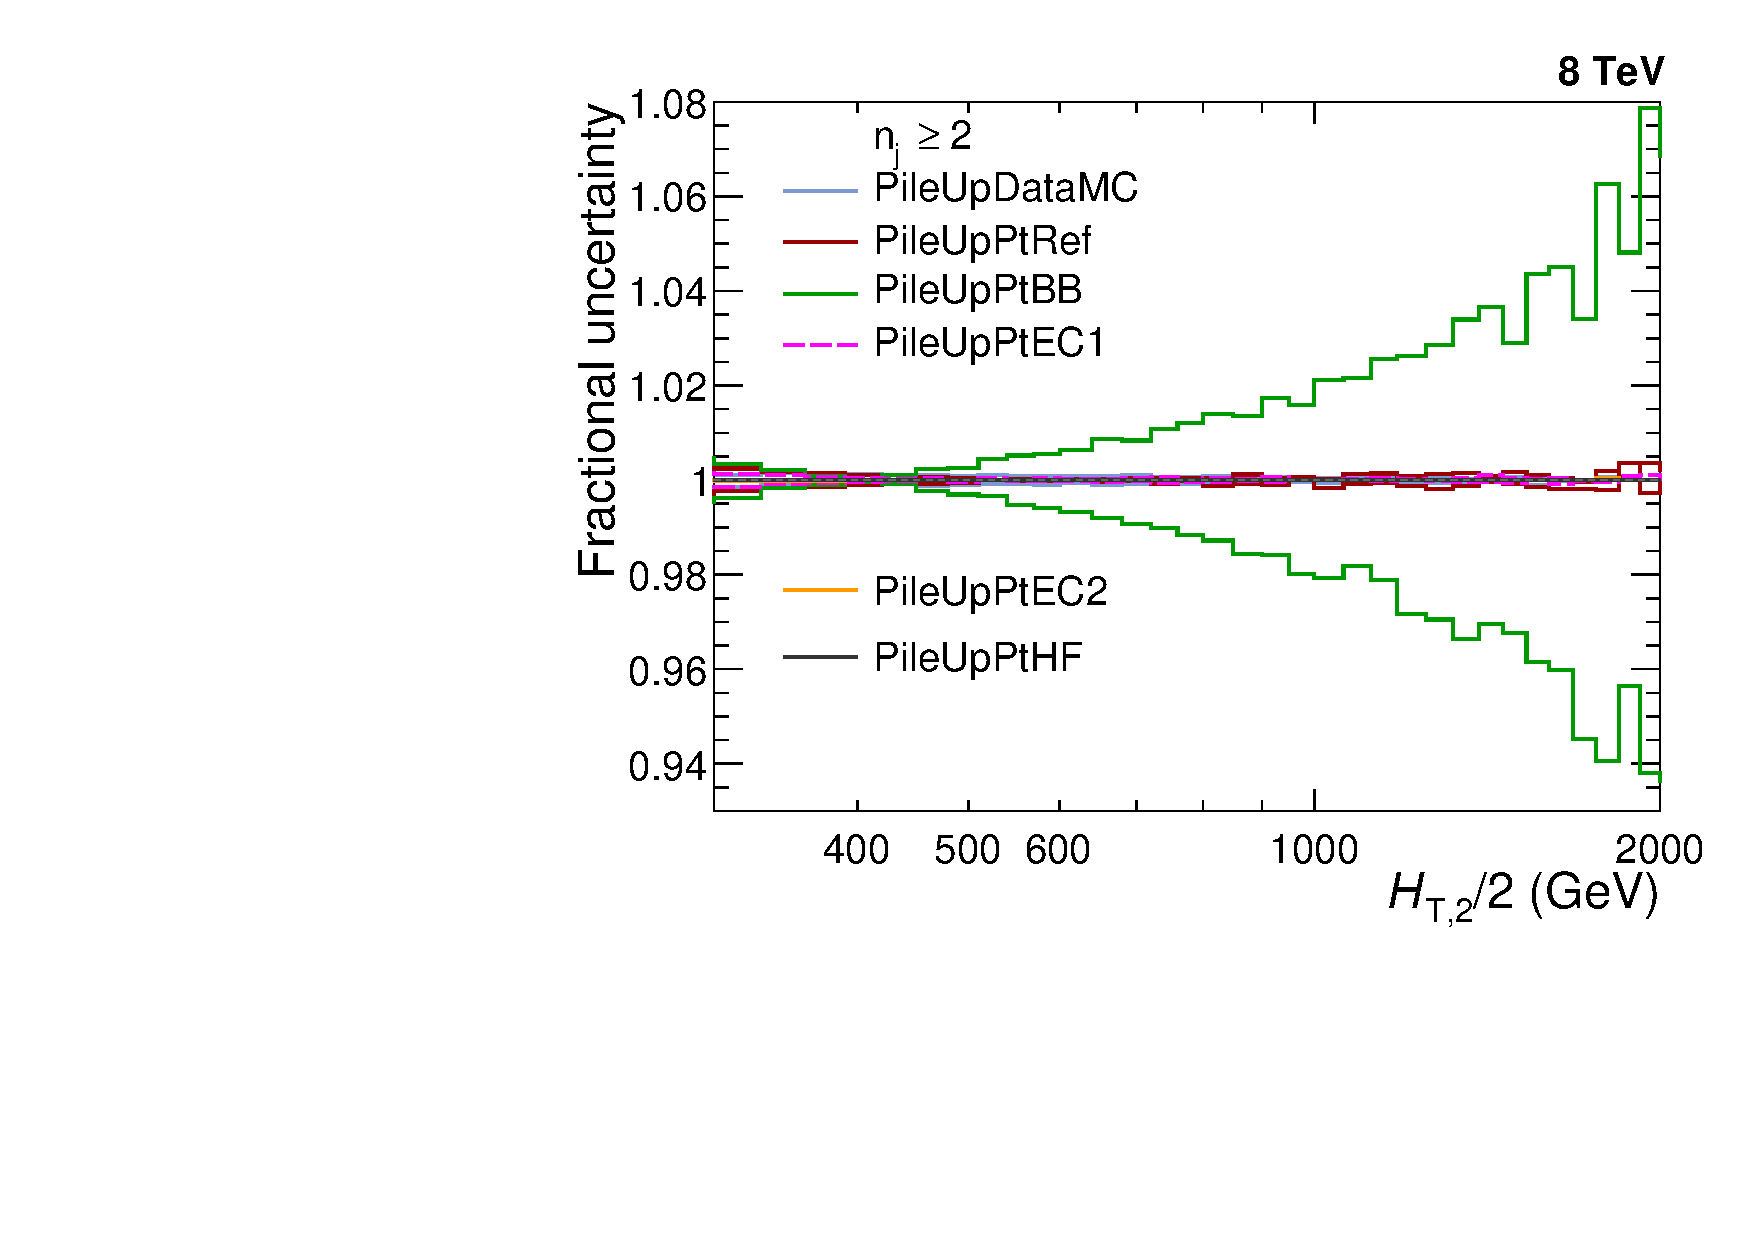
\includegraphics[width=0.51\textwidth]{/home/anter/Desktop/Thesis/Plots_HT_2_150/Single/MC_Macro_Plot_All_3_HT_2_Unc_Pileup_1.pdf}\\
\hspace*{-5mm}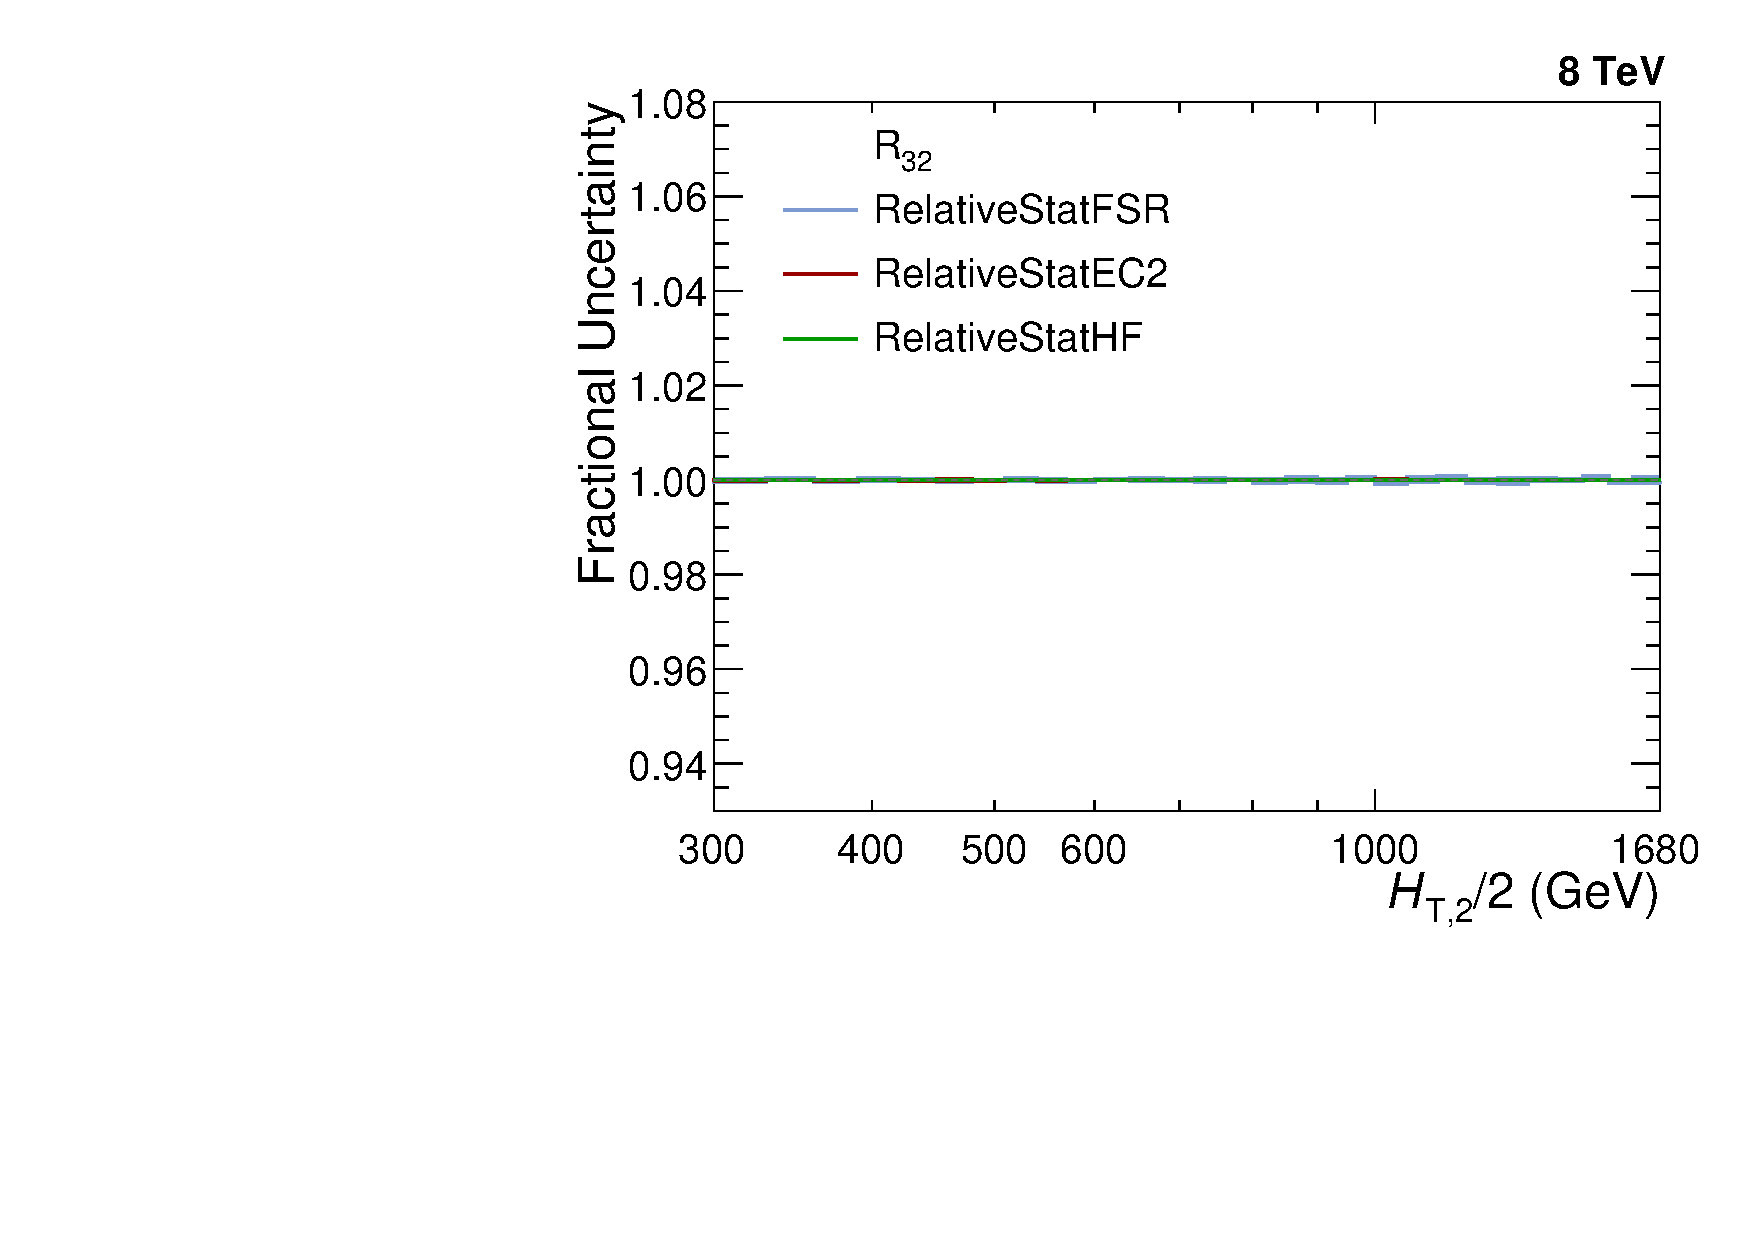
\includegraphics[width=0.51\textwidth]{/home/anter/Desktop/Thesis/Plots_HT_2_150/Single/MC_Macro_Plot_Ratio_32_HT_2_Unc_RelativeStat_1.pdf}%
~~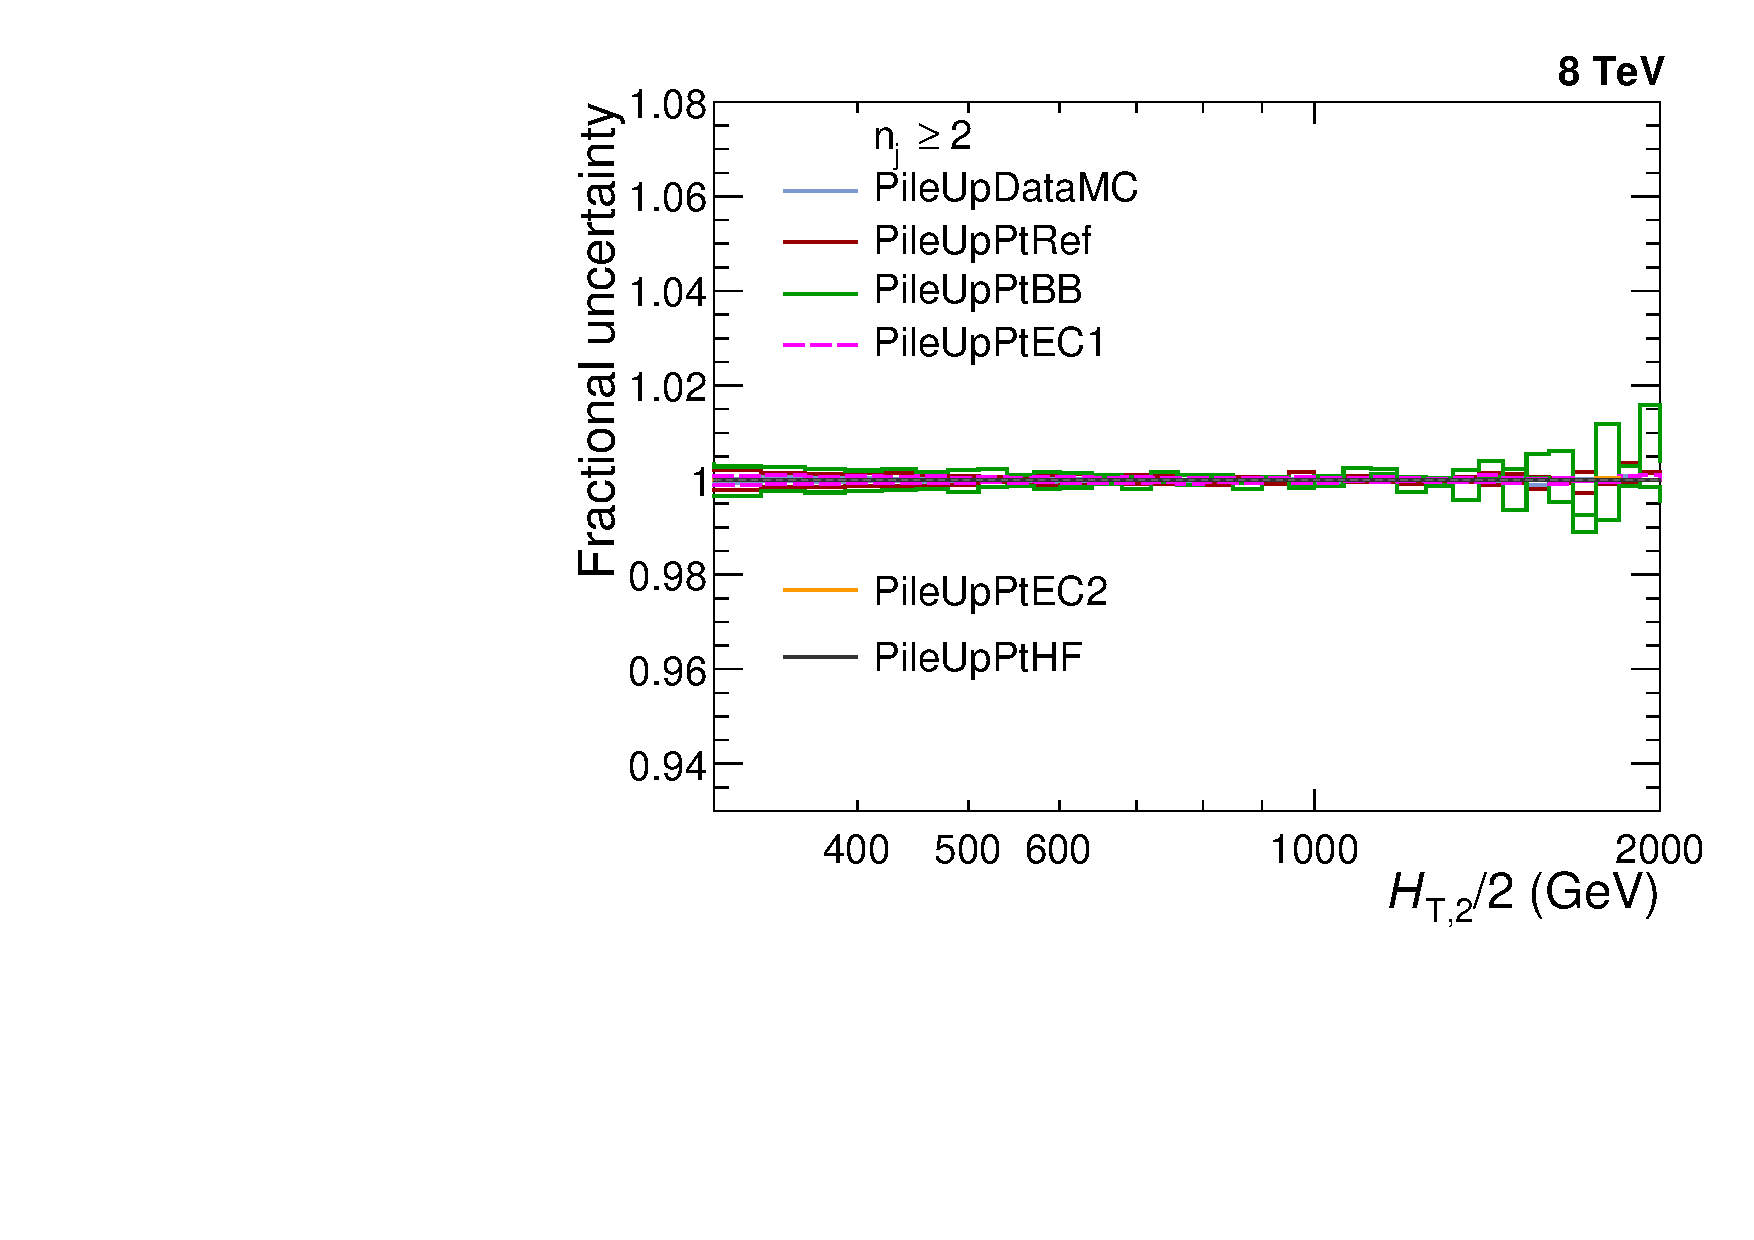
\includegraphics[width=0.51\textwidth]{/home/anter/Desktop/Thesis/Plots_HT_2_150/Single/MC_Macro_Plot_Ratio_32_HT_2_Unc_Pileup_1.pdf}\\
\caption{The relative size of the jet energy correction (JEC) uncertainties for individual sources are shown for inclusive 2-jet (top) and 3-jet events cross sections (middle); and cross section ratio \ratio (bottom). On left, JEC uncertainties are evaluated from \textcolor{blue2}{RelativeStatFSR}, \textcolor{red}{RelativeStatEC2} and \textcolor{green}{RelativeStatHF} sources whereas on right, these are evaluated from \textcolor{blue2}{PileUpDataMC}, \textcolor{red}{PileUpPtRef}, \textcolor{green}{PileUpPtBB}, \textcolor{pink2}{PileUpPtEC1}, \textcolor{deepsaffron}{PileUpPtEC2} and \textcolor{dimgray}{PileUpPtHF} sources.}
\label{fig:jes3}
%\end{center}
\end{figure}

\section{Experimental uncertainties}
\label{sec:Exp_unc}
\begin{table}[!htbp]
  \caption{Bin-wise values (in \%) of all experimental uncertainties affecting the cross section measurement for inclusive 2-jet events.}
  \label{tab:exp_unc2}
  \centering
  \vspace{2mm}
  \begin{tabular}{ccccccc} \hline \hline
    %&  x-section  &  &  & &  & &  \rbtrrn \\ 
    %Bin  &  (x 10$^{-3}$ (pb/GeV))   & {\bf Statistical} & {\bf \textcolor{blue}{JEC}} & {\bf \textcolor{green} {Unfolding}} & {\bf \textcolor{red}{Lumi}} & {\bf \textcolor{lightpurple} {Residual}} & {\bf Total} \rbtrrn \\  \hline 
    Bin  &  {\bf Statistical} & {\bf \textcolor{blue2}{JEC}} & {\bf \textcolor{green} {Unfolding}} & {\bf \textcolor{red}{Lumi}} & {\bf \textcolor{lightpurple} {Residual}} & {\bf Total} \rbtrrn \\  \hline 
    
300 - 330 & 0.242 & $^{+2.612}_{-2.565}$ & $^{+0.948}_{-0.928}$ &  2.6 &  1.0 & $^{+3.942}_{-3.906}$ \rbtrrn \\ \hline
330 - 360 & 0.258 & $^{+2.507}_{-2.473}$ & $^{+0.976}_{-0.969}$ &  2.6 &  1.0 & $^{+3.882}_{-3.858}$ \rbtrrn \\ \hline
360 - 390 & 0.202 & $^{+2.504}_{-2.465}$ & $^{+0.779}_{-0.783}$ &  2.6 &  1.0 & $^{+3.831}_{-3.807}$ \rbtrrn \\ \hline
390 - 420 & 0.193 & $^{+2.363}_{-2.381}$ & $^{+0.905}_{-0.904}$ &  2.6 &  1.0 & $^{+3.768}_{-3.780}$ \rbtrrn \\ \hline
420 - 450 & 0.084 & $^{+2.448}_{-2.422}$ & $^{+0.904}_{-0.895}$ &  2.6 &  1.0 & $^{+3.818}_{-3.799}$ \rbtrrn \\ \hline
450 - 480 & 0.096 & $^{+2.440}_{-2.352}$ & $^{+0.797}_{-0.795}$ &  2.6 &  1.0 & $^{+3.789}_{-3.733}$ \rbtrrn \\ \hline
480 - 510 & 0.107 & $^{+2.427}_{-2.406}$ & $^{+0.728}_{-0.715}$ &  2.6 &  1.0 & $^{+3.767}_{-3.751}$ \rbtrrn \\ \hline
510 - 540 & 0.128 & $^{+2.425}_{-2.395}$ & $^{+0.835}_{-0.862}$ &  2.6 &  1.0 & $^{+3.789}_{-3.775}$ \rbtrrn \\ \hline
540 - 570 & 0.154 & $^{+2.425}_{-2.376}$ & $^{+0.687}_{-0.674}$ &  2.6 &  1.0 & $^{+3.760}_{-3.726}$ \rbtrrn \\ \hline
570 - 600 & 0.180 & $^{+2.497}_{-2.474}$ & $^{+0.839}_{-0.827}$ &  2.6 &  1.0 & $^{+3.838}_{-3.820}$ \rbtrrn \\ \hline
600 - 640 & 0.209 & $^{+2.495}_{-2.491}$ & $^{+0.744}_{-0.743}$ &  2.6 &  1.0 & $^{+3.819}_{-3.816}$ \rbtrrn \\ \hline
640 - 680 & 0.264 & $^{+2.582}_{-2.545}$ & $^{+0.912}_{-0.912}$ &  2.6 &  1.0 & $^{+3.915}_{-3.891}$ \rbtrrn \\ \hline
680 - 720 & 0.320 & $^{+2.691}_{-2.574}$ & $^{+0.763}_{-0.756}$ &  2.6 &  1.0 & $^{+3.961}_{-3.880}$ \rbtrrn \\ \hline
720 - 760 & 0.387 & $^{+2.690}_{-2.755}$ & $^{+0.705}_{-0.712}$ &  2.6 &  1.0 & $^{+3.955}_{-4.001}$ \rbtrrn \\ \hline
760 - 800 & 0.465 & $^{+2.858}_{-2.846}$ & $^{+0.859}_{-0.846}$ &  2.6 &  1.0 & $^{+4.109}_{-4.098}$ \rbtrrn \\ \hline
800 - 850 & 0.548 & $^{+2.889}_{-2.913}$ & $^{+0.783}_{-0.787}$ &  2.6 &  1.0 & $^{+4.126}_{-4.143}$ \rbtrrn \\ \hline
850 - 900 & 0.698 & $^{+3.145}_{-3.102}$ & $^{+0.961}_{-0.958}$ &  2.6 &  1.0 & $^{+4.366}_{-4.334}$ \rbtrrn \\ \hline
900 - 950 & 0.847 & $^{+3.298}_{-3.233}$ & $^{+0.828}_{-0.829}$ &  2.6 &  1.0 & $^{+4.476}_{-4.429}$ \rbtrrn \\ \hline
950 - 1000 & 1.041 & $^{+3.291}_{-3.330}$ & $^{+0.895}_{-0.872}$ &  2.6 &  1.0 & $^{+4.525}_{-4.549}$ \rbtrrn \\ \hline
1000 - 1060 & 1.268 & $^{+3.598}_{-3.569}$ & $^{+0.945}_{-0.956}$ &  2.6 &  1.0 & $^{+4.817}_{-4.798}$ \rbtrrn \\ \hline
1060 - 1120 & 1.611 & $^{+3.759}_{-3.756}$ & $^{+0.970}_{-0.967}$ &  2.6 &  1.0 & $^{+5.043}_{-5.040}$ \rbtrrn \\ \hline
1120 - 1180 & 1.985 & $^{+4.154}_{-4.053}$ & $^{+1.089}_{-1.080}$ &  2.6 &  1.0 & $^{+5.490}_{-5.413}$ \rbtrrn \\ \hline
1180 - 1250 & 2.406 & $^{+4.251}_{-4.313}$ & $^{+1.062}_{-1.070}$ &  2.6 &  1.0 & $^{+5.722}_{-5.770}$ \rbtrrn \\ \hline
1250 - 1320 & 3.101 & $^{+4.696}_{-4.624}$ & $^{+1.151}_{-1.144}$ &  2.6 &  1.0 & $^{+6.384}_{-6.330}$ \rbtrrn \\ \hline
1320 - 1390 & 4.157 & $^{+4.934}_{-4.979}$ & $^{+1.343}_{-1.341}$ &  2.6 &  1.0 & $^{+7.155}_{-7.186}$ \rbtrrn \\ \hline
1390 - 1460 & 5.270 & $^{+5.148}_{-5.104}$ & $^{+1.185}_{-1.177}$ &  2.6 &  1.0 & $^{+7.965}_{-7.936}$ \rbtrrn \\ \hline
1460 - 1530 & 6.360 & $^{+5.890}_{-5.652}$ & $^{+1.405}_{-1.406}$ &  2.6 &  1.0 & $^{+9.213}_{-9.063}$ \rbtrrn \\ \hline
1530 - 1600 & 8.183 & $^{+5.924}_{-6.311}$ & $^{+1.598}_{-1.590}$ &  2.6 &  1.0 & $^{+10.601}_{-10.821}$ \rbtrrn \\ \hline
1600 - 1680 & 10.630 & $^{+5.969}_{-5.655}$ & $^{+1.607}_{-1.592}$ &  2.6 &  1.0 & $^{+12.608}_{-12.461}$ \rbtrrn \\ \hline
1680 - 1760 & 13.864 & $^{+7.245}_{-7.603}$ & $^{+1.821}_{-1.839}$ &  2.6 &  1.0 & $^{+15.993}_{-16.161}$ \rbtrrn \\ \hline
1760 - 1840 & 18.192 & $^{+7.781}_{-7.820}$ & $^{+1.902}_{-1.906}$ &  2.6 &  1.0 & $^{+20.071}_{-20.087}$ \rbtrrn \\ \hline
1840 - 1920 & 22.612 & $^{+7.647}_{-7.537}$ & $^{+1.588}_{-1.590}$ &  2.6 &  1.0 & $^{+24.085}_{-24.050}$ \rbtrrn \\ \hline
1920 - 2000 & 29.530 & $^{+9.199}_{-9.469}$ & $^{+1.511}_{-1.505}$ &  2.6 &  1.0 & $^{+31.092}_{-31.172}$ \rbtrrn \\ \hline
 \hline
 \end{tabular}
\end{table}

\begin{table}[!htbp]
  \caption{Bin-wise values (in \%) of all experimental uncertainties affecting the cross section measurement for inclusive 3-jet events.}
  \label{tab:exp_unc3}
  \centering
  \vspace{2mm}
  \begin{tabular}{ccccccc} \hline \hline
    %&  x-section  &  &  & &  & &  \rbtrrn \\ 
    %Bin  &  (x 10$^{-3}$ (pb/GeV))   & {\bf Statistical} & {\bf \textcolor{blue}{JEC}} & {\bf \textcolor{green} {Unfolding}} & {\bf \textcolor{red}{Lumi}} & {\bf \textcolor{lightpurple} {Residual}} & {\bf Total} \rbtrrn \\  \hline 
    Bin  &  {\bf Statistical} & {\bf \textcolor{blue2}{JEC}} & {\bf \textcolor{green} {Unfolding}} & {\bf \textcolor{red}{Lumi}} & {\bf \textcolor{lightpurple} {Residual}} & {\bf Total} \rbtrrn \\  \hline 

300 - 330 & 0.796 & $^{+3.503}_{-3.475}$ & $^{+0.564}_{-0.552}$ &  2.6 &  1.0 & $^{+4.581}_{-4.558}$ \rbtrrn \\ \hline
330 - 360 & 0.781 & $^{+3.303}_{-3.186}$ & $^{+0.640}_{-0.633}$ &  2.6 &  1.0 & $^{+4.437}_{-4.350}$ \rbtrrn \\ \hline
360 - 390 & 0.583 & $^{+3.221}_{-3.094}$ & $^{+0.490}_{-0.496}$ &  2.6 &  1.0 & $^{+4.326}_{-4.233}$ \rbtrrn \\ \hline
390 - 420 & 0.531 & $^{+3.092}_{-3.149}$ & $^{+0.584}_{-0.584}$ &  2.6 &  1.0 & $^{+4.236}_{-4.278}$ \rbtrrn \\ \hline
420 - 450 & 0.224 & $^{+3.125}_{-2.996}$ & $^{+0.604}_{-0.592}$ &  2.6 &  1.0 & $^{+4.236}_{-4.140}$ \rbtrrn \\ \hline
450 - 480 & 0.248 & $^{+2.984}_{-2.890}$ & $^{+0.531}_{-0.528}$ &  2.6 &  1.0 & $^{+4.124}_{-4.056}$ \rbtrrn \\ \hline
480 - 510 & 0.269 & $^{+2.937}_{-2.963}$ & $^{+0.511}_{-0.512}$ &  2.6 &  1.0 & $^{+4.089}_{-4.108}$ \rbtrrn \\ \hline
510 - 540 & 0.318 & $^{+3.021}_{-2.797}$ & $^{+0.592}_{-0.612}$ &  2.6 &  1.0 & $^{+4.164}_{-4.007}$ \rbtrrn \\ \hline
540 - 570 & 0.375 & $^{+2.999}_{-2.935}$ & $^{+0.506}_{-0.500}$ &  2.6 &  1.0 & $^{+4.141}_{-4.094}$ \rbtrrn \\ \hline
570 - 600 & 0.434 & $^{+2.824}_{-2.906}$ & $^{+0.646}_{-0.620}$ &  2.6 &  1.0 & $^{+4.042}_{-4.096}$ \rbtrrn \\ \hline
600 - 640 & 0.497 & $^{+2.952}_{-2.956}$ & $^{+0.598}_{-0.604}$ &  2.6 &  1.0 & $^{+4.133}_{-4.136}$ \rbtrrn \\ \hline
640 - 680 & 0.617 & $^{+3.111}_{-3.001}$ & $^{+0.777}_{-0.786}$ &  2.6 &  1.0 & $^{+4.292}_{-4.215}$ \rbtrrn \\ \hline
680 - 720 & 0.739 & $^{+3.067}_{-2.984}$ & $^{+0.642}_{-0.611}$ &  2.6 &  1.0 & $^{+4.257}_{-4.194}$ \rbtrrn \\ \hline
720 - 760 & 0.895 & $^{+3.185}_{-3.111}$ & $^{+0.595}_{-0.607}$ &  2.6 &  1.0 & $^{+4.366}_{-4.313}$ \rbtrrn \\ \hline
760 - 800 & 1.068 & $^{+3.231}_{-3.166}$ & $^{+0.763}_{-0.774}$ &  2.6 &  1.0 & $^{+4.464}_{-4.419}$ \rbtrrn \\ \hline
800 - 850 & 1.250 & $^{+3.427}_{-3.295}$ & $^{+0.674}_{-0.687}$ &  2.6 &  1.0 & $^{+4.639}_{-4.544}$ \rbtrrn \\ \hline
850 - 900 & 1.578 & $^{+3.364}_{-3.540}$ & $^{+0.903}_{-0.898}$ &  2.6 &  1.0 & $^{+4.731}_{-4.857}$ \rbtrrn \\ \hline
900 - 950 & 1.961 & $^{+3.594}_{-3.524}$ & $^{+0.792}_{-0.793}$ &  2.6 &  1.0 & $^{+5.015}_{-4.965}$ \rbtrrn \\ \hline
950 - 1000 & 2.420 & $^{+3.603}_{-3.783}$ & $^{+0.846}_{-0.843}$ &  2.6 &  1.0 & $^{+5.226}_{-5.351}$ \rbtrrn \\ \hline
1000 - 1060 & 2.844 & $^{+4.164}_{-4.116}$ & $^{+0.916}_{-0.940}$ &  2.6 &  1.0 & $^{+5.834}_{-5.803}$ \rbtrrn \\ \hline
1060 - 1120 & 3.647 & $^{+4.038}_{-3.815}$ & $^{+0.963}_{-0.957}$ &  2.6 &  1.0 & $^{+6.188}_{-6.044}$ \rbtrrn \\ \hline
1120 - 1180 & 4.607 & $^{+4.278}_{-4.183}$ & $^{+1.084}_{-1.087}$ &  2.6 &  1.0 & $^{+6.961}_{-6.904}$ \rbtrrn \\ \hline
1180 - 1250 & 5.532 & $^{+4.894}_{-4.771}$ & $^{+1.074}_{-1.069}$ &  2.6 &  1.0 & $^{+7.967}_{-7.891}$ \rbtrrn \\ \hline
1250 - 1320 & 7.141 & $^{+5.144}_{-5.273}$ & $^{+1.222}_{-1.217}$ &  2.6 &  1.0 & $^{+9.312}_{-9.383}$ \rbtrrn \\ \hline
1320 - 1390 & 10.207 & $^{+5.542}_{-5.642}$ & $^{+1.414}_{-1.428}$ &  2.6 &  1.0 & $^{+12.027}_{-12.076}$ \rbtrrn \\ \hline
1390 - 1460 & 13.831 & $^{+5.630}_{-5.265}$ & $^{+1.257}_{-1.256}$ &  2.6 &  1.0 & $^{+15.242}_{-15.111}$ \rbtrrn \\ \hline
1460 - 1530 & 15.578 & $^{+5.576}_{-5.491}$ & $^{+1.546}_{-1.551}$ &  2.6 &  1.0 & $^{+16.850}_{-16.822}$ \rbtrrn \\ \hline
1530 - 1600 & 18.729 & $^{+6.409}_{-7.019}$ & $^{+1.718}_{-1.716}$ &  2.6 &  1.0 & $^{+20.063}_{-20.266}$ \rbtrrn \\ \hline
1600 - 1680 & 26.465 & $^{+7.017}_{-6.255}$ & $^{+1.775}_{-1.765}$ &  2.6 &  1.0 & $^{+27.578}_{-27.393}$ \rbtrrn \\ \hline
   \hline
  \end{tabular}
\end{table}


\begin{table}[!htbp]
  \caption{Bin-wise values (in \%) of all experimental uncertainties affecting the measurement of cross section ratio \ratio.}
  \label{tab:exp_unc_ratio}
  \centering
  \vspace{2mm}
  \begin{tabular}{cccccc} \hline \hline
    %Bin  &  \ratio   & {\bf Statistical } & {\bf \blue {JEC}} & {\bf \textcolor{green!50!black} {Unfolding}}  & {\bf Total} \rbtrrn \\ \hline 
    Bin  &  {\bf Statistical} & {\bf \textcolor{blue2}{JEC}} & {\bf \textcolor{green} {Unfolding}} & {\bf Total} \rbtrrn \\  \hline 
300 - 330 & 0.741 & $^{+1.059}_{-1.097}$ & $^{+0.754}_{-0.751}$ & $^{+1.496}_{-1.522}$ \rbtrrn \\ \hline
330 - 360 & 0.587 & $^{+0.954}_{-0.923}$ & $^{+0.685}_{-0.689}$ & $^{+1.313}_{-1.292}$ \rbtrrn \\ \hline
360 - 390 & 0.519 & $^{+0.902}_{-0.855}$ & $^{+0.594}_{-0.593}$ & $^{+1.199}_{-1.163}$ \rbtrrn \\ \hline
390 - 420 & 0.236 & $^{+0.907}_{-0.952}$ & $^{+0.439}_{-0.438}$ & $^{+1.035}_{-1.074}$ \rbtrrn \\ \hline
420 - 450 & 0.192 & $^{+0.900}_{-0.835}$ & $^{+0.360}_{-0.361}$ & $^{+0.988}_{-0.930}$ \rbtrrn \\ \hline
450 - 480 & 0.209 & $^{+0.788}_{-0.802}$ & $^{+0.307}_{-0.308}$ & $^{+0.872}_{-0.884}$ \rbtrrn \\ \hline
480 - 510 & 0.245 & $^{+0.795}_{-0.867}$ & $^{+0.254}_{-0.235}$ & $^{+0.870}_{-0.931}$ \rbtrrn \\ \hline
510 - 540 & 0.287 & $^{+0.852}_{-0.682}$ & $^{+0.264}_{-0.268}$ & $^{+0.937}_{-0.787}$ \rbtrrn \\ \hline
540 - 570 & 0.326 & $^{+0.807}_{-0.803}$ & $^{+0.193}_{-0.189}$ & $^{+0.891}_{-0.887}$ \rbtrrn \\ \hline
570 - 600 & 0.397 & $^{+0.656}_{-0.774}$ & $^{+0.199}_{-0.219}$ & $^{+0.792}_{-0.898}$ \rbtrrn \\ \hline
600 - 640 & 0.447 & $^{+0.763}_{-0.797}$ & $^{+0.150}_{-0.154}$ & $^{+0.897}_{-0.926}$ \rbtrrn \\ \hline
640 - 680 & 0.573 & $^{+0.861}_{-0.781}$ & $^{+0.153}_{-0.140}$ & $^{+1.045}_{-0.979}$ \rbtrrn \\ \hline
680 - 720 & 0.663 & $^{+0.766}_{-0.787}$ & $^{+0.147}_{-0.164}$ & $^{+1.024}_{-1.042}$ \rbtrrn \\ \hline
720 - 760 & 0.774 & $^{+0.842}_{-0.769}$ & $^{+0.118}_{-0.118}$ & $^{+1.149}_{-1.097}$ \rbtrrn \\ \hline
760 - 800 & 0.970 & $^{+0.800}_{-0.729}$ & $^{+0.115}_{-0.096}$ & $^{+1.263}_{-1.218}$ \rbtrrn \\ \hline
800 - 850 & 1.116 & $^{+0.873}_{-0.775}$ & $^{+0.115}_{-0.104}$ & $^{+1.422}_{-1.363}$ \rbtrrn \\ \hline
850 - 900 & 1.436 & $^{+0.770}_{-0.896}$ & $^{+0.069}_{-0.069}$ & $^{+1.631}_{-1.694}$ \rbtrrn \\ \hline
900 - 950 & 1.716 & $^{+0.704}_{-0.752}$ & $^{+0.050}_{-0.051}$ & $^{+1.855}_{-1.874}$ \rbtrrn \\ \hline
950 - 1000 & 2.156 & $^{+0.824}_{-0.897}$ & $^{+0.089}_{-0.045}$ & $^{+2.310}_{-2.336}$ \rbtrrn \\ \hline
1000 - 1060 & 2.554 & $^{+0.812}_{-0.870}$ & $^{+0.045}_{-0.040}$ & $^{+2.680}_{-2.698}$ \rbtrrn \\ \hline
1060 - 1120 & 3.244 & $^{+0.792}_{-0.658}$ & $^{+0.018}_{-0.027}$ & $^{+3.339}_{-3.310}$ \rbtrrn \\ \hline
1120 - 1180 & 4.121 & $^{+0.985}_{-0.757}$ & $^{+0.025}_{-0.043}$ & $^{+4.237}_{-4.191}$ \rbtrrn \\ \hline
1180 - 1250 & 4.990 & $^{+1.031}_{-0.848}$ & $^{+0.023}_{-0.041}$ & $^{+5.095}_{-5.062}$ \rbtrrn \\ \hline
1250 - 1320 & 6.456 & $^{+0.750}_{-1.087}$ & $^{+0.079}_{-0.079}$ & $^{+6.500}_{-6.548}$ \rbtrrn \\ \hline
1320 - 1390 & 8.990 & $^{+1.112}_{-1.144}$ & $^{+0.080}_{-0.099}$ & $^{+9.059}_{-9.063}$ \rbtrrn \\ \hline
1390 - 1460 & 12.699 & $^{+1.157}_{-0.815}$ & $^{+0.076}_{-0.078}$ & $^{+12.751}_{-12.725}$ \rbtrrn \\ \hline
1460 - 1530 & 13.926 & $^{+0.768}_{-1.235}$ & $^{+0.143}_{-0.145}$ & $^{+13.948}_{-13.981}$ \rbtrrn \\ \hline
1530 - 1600 & 16.903 & $^{+1.050}_{-1.258}$ & $^{+0.120}_{-0.127}$ & $^{+16.936}_{-16.950}$ \rbtrrn \\ \hline
1600 - 1680 & 28.070 & $^{+1.471}_{-0.859}$ & $^{+0.178}_{-0.177}$ & $^{+28.109}_{-28.084}$ \rbtrrn \\ \hline
 \hline
 \end{tabular}
\end{table}
